% !TeX spellcheck = it_IT
%%%%%%%%%%%%%%%%%%%%%%%%%%%%%%%%%%%%%%%%%%%%%%%%%%%%%%%%%%%%%%%%%%%%%%%%%%%%%%%%%%%%%%%%%%%%%%%%%%%%%%%%
%Paolo Eccher, Andrea Favero, Cristian Maschio, Francesco Parolini
%%%%%%%%%%%%%%%%%%%%%%%%%%%%%%%%%%%%%%%%%%%%%%%%%%%%%%%%%%%%%%%%%%%%%%%%%%%%%%%%%%%%%%%%%%%%%%%%%%%%%%%%

\documentclass[10pt, a4paper]{article}

\usepackage[scaled]{helvet}

\usepackage[utf8]{inputenc}
\usepackage[T1]{fontenc}
\usepackage[italian]{babel}

\usepackage{graphicx}
\usepackage{fix-cm}
\newcommand{\bigsize}{\fontsize{35pt}{20pt}\selectfont}
\newcommand{\mediumsize}{\fontsize{30pt}{20pt}\selectfont}
\newcommand{\normsize}{\fontsize{15pt}{10pt}\selectfont}

%\usepackage{marginnote} %note a margine della pagina

%crea uno spazio, utile perchè gli spazi extra dopo le macro
%vengono rimossi. Questo comando permette di inserirne uno.
\def\space{ }

\usepackage{float}
\usepackage{caption}

\usepackage{amsmath}
\usepackage{mathtools}

\usepackage{multirow}
%crea una cella per le tabelle in grado di andare a capo con \newline
%https://tex.stackexchange.com/questions/12703/how-to-create-fixed-width-table-columns-with-text-raggedright-centered-raggedlef
\usepackage{array}
\newcolumntype{L}[1]{>{\raggedright\let\newline\\\arraybackslash\hspace{0pt}}m{#1}}
\newcolumntype{C}[1]{>{\centering\let\newline\\\arraybackslash\hspace{0pt}}m{#1}}
\newcolumntype{R}[1]{>{\raggedleft\let\newline\\\arraybackslash\hspace{0pt}}m{#1}}

%puntini per l'indice
\usepackage{tocloft}
\renewcommand\cftsecleader{\cftdotfill{\cftdotsep}}


%https://tex.stackexchange.com/questions/4503/how-do-i-specify-color-in-rgb-using-hypersetup-in-hyperref
\usepackage{url}
\usepackage{breakurl}
\usepackage[colorlinks=true]{hyperref}
\usepackage[hyperref]{xcolor}
\definecolor{UniPD}{RGB}{155, 0, 20}
\definecolor{Crema}{RGB}{220, 197, 149}
\definecolor{LinkNormNoClick}{RGB}{0, 0, 238}
\definecolor{LinkNormClick}{RGB}{69, 123, 157}
\hypersetup{colorlinks,breaklinks,
	urlcolor=UniPD,
	linkcolor=UniPD}

%per alcune liste
\usepackage{blindtext}
\usepackage{scrextend}
\addtokomafont{labelinglabel}
{\sffamily}


\newcommand{\Componenti}{Paolo Eccher \newline Cristian Maschio \newline
	Andrea Favero \newline Francesco Parolini}
\newcommand{\Referente}{Andrea Favero \newline andrea.favero.8@studenti.unipd.it}
\newcommand{\Gruppo}{Eccher, Maschio, Favero, Parolini}
\newcommand{\Titolo}{Progetto tecnologie web}

\usepackage{lastpage} %info sul # dell'ultima pagina del documento
\usepackage{fancyhdr} %per modificare dimensioni,margini, intestazioni e righe a piè di pagina
\fancypagestyle{plain}{
	% cancella tutti i campi di intestazione e piè di pagina
	\fancyhf{}
	
	\lfoot{ %piè di pagina
		\Titolo{} \ - \textit{\Gruppo{}}
	}
	\rfoot{Pagina \thepage{} di \pageref{LastPage}} %es: pag: 4 di 10
	
	%linea orizzontale alle posizioni top e bottom della pagina
	\renewcommand{\headrulewidth}{0pt}  
	\renewcommand{\footrulewidth}{0.3pt}
}
\pagestyle{plain}

\usepackage{manfnt} %%per cartelli stradali knuth/bourbaki. da togliere

%%%%%%%%%%%%%%%%%%%%%%%%%%%%%%%%%%%%%%%%%%%%%%%%%%%%%%%%%%%%%%%%%%%%%%%%%%
%%%%%%%%%%%%%%%%%%%%%%%%%%%%%%%%%%%%%%%%%%%%%%%%%%%%%%%%%%%%%%%%%%%%%%%%%%
%%%%%%%%%%%%%%%%%%%%%%%%%%%%%%%%%%%%%%%%%%%%%%%%%%%%%%%%%%%%%%%%%%%%%%%%%%
%%%    SNIPPET html monokai theme
%%%%%%%%%%%%%%%%%%%%%%%%%%%%%%%%%%%%%%%%%%%%%%%%%%%%%%%%%%%%%%%%%%%%%%%%%%
%%%%%%%%%%%%%%%%%%%%%%%%%%%%%%%%%%%%%%%%%%%%%%%%%%%%%%%%%%%%%%%%%%%%%%%%%%


\usepackage{listings}

\definecolor{background}{RGB}{46, 46, 46}  %%nero
\definecolor{string}{RGB}{230, 219, 116} %%giallo
\definecolor{comment}{RGB}{117, 113, 94} %%grey
\definecolor{normal}{RGB}{248, 248, 242} %%bianco
\definecolor{purple}{RGB}{242, 16, 114} %%purple
\definecolor{identifier}{RGB}{166, 226, 46} %%verde
\definecolor{blue}{RGB}{0, 102, 255}


\lstdefinelanguage{HTML5}{
	sensitive=true,
	keywords={
		%% JavaScript
		typeof, new, true, false, catch, function, return, null, catch, switch, var, if, in, while, do, else, case, break, foreach, as,
		%% HTML
		html, meta, style, head, body, script, canvas, h1, h2, h3, h4, h5, h6, table, thead, tbody, tfoot, p, a, div, input, form, tr, th, label, ?php, ?, 
		%% CSS
		border:, transform:, -moz-transform:, transition-duration:, transition-property:,
		transition-timing-function:
	},
	% http://texblog.org/tag/otherkeywords/
	keywords=[2]{<, >, \, /, />, </ },  %%tag
	keywords=[3]{href, title, label, aria-label, lang, for, tabindex, placeholder, id, type, value, class, scope, }, %%attributi
	ndkeywords={class, export, boolean, throw, implements, import, this},
	keywords=[4]{echo, print\_ordinable\_th, REQUIRED},
	comment=[l]{//},
	% morecomment=[s][keywordstyle]{<}{>},  
	morecomment=[s]{/*}{*/},
	morecomment=[s]{<!}{>},
	morestring=[b]',
	morestring=[b]",    
	alsoletter={-},
	alsodigit={:}
}

\lstset{
	backgroundcolor=\color{background},
	tabsize=4,    
	language=HTML5,
	basicstyle=\ttfamily\linespread{1.15}\footnotesize,
	upquote=true,
	aboveskip={1.5},
	columns=fixed,
	showstringspaces=false,
	extendedchars=true,
	inputencoding=utf8,
	breaklines=true,
	prebreak = \raisebox{0ex}[0ex][0ex]{\ensuremath{\hookleftarrow}},
	frame=none,
	numbers=left,
	numbersep=5pt,	
	showtabs=false,
	showspaces=false,
	showstringspaces=false,
	basicstyle=\tiny\color{normal},
	identifierstyle=\color{normal},
	keywordstyle=\color{purple},
	keywordstyle=[2]\color{normal},
	keywordstyle=[3]\color{identifier},
	keywordstyle=[4]\color{blue},
	commentstyle=\color{comment},
	stringstyle=\color{string},
	numberstyle=\tiny\color{background}.
}

%%%%%%%%%%%%%%%%%%%%%%%%%%%%%%%%%%%%%%%%%%%%%%%%%%%%%%%%%%%%%%%%%%%%%%%%%%%%%%%%%%%%%%%%%%%%%%%%%%%%%%%%

\begin{document}

%%%%%%%%%%%%%%%%%%%%%%%%%%%%%%%%%%%%%%%%%%%%%%%%%%%%%%%%%%%%%%%%%%%%%%%%%%%%%%%%%%%%%%%%%%%%%%%%%%%%%%%%
\begin{titlepage}
\centering


\includegraphics[width=50mm]{Images/logo.png}
\vspace*{32px}
{\Large \\ \textbf{RELAZIONE}\\}
\vspace*{2px}
{\Large \textbf{TECNOLOGIE WEB}\\}
\vspace*{27px}

\bgroup
\def\arraystretch{1.3}
\centering
\begin{tabular}{c|L{5cm}}
\multicolumn{2}{c}{\textbf{gruppo} } \\ \hline
  Componenti & \Componenti{} \\
  Referente & \Referente{}
\end{tabular}
\egroup

\vspace*{8px}

\bgroup
\def\arraystretch{1.3}
\centering
\begin{tabular}{c}
\multicolumn{1}{c}{\textbf{Indirizzo web del sito} } \\
  \url{http://tecweb.studenti.math.unipd.it/anfavero}
\end{tabular}
\egroup

\vspace*{10px}

\begin{tabular}{c|L{3cm}}
\multicolumn{2}{c}{\textbf{Credenziali admin} } \\ \hline
  Username & admin \\
  Password & admin
\end{tabular}
\quad
\begin{tabular}{c|L{3cm}}
\multicolumn{2}{c}{\textbf{Credenziali utente semplice} } \\ \hline
  Username & user \\
  Password & user
\end{tabular}
\vspace*{8px}
\begin{tabular}{c|L{3cm}}
	\multicolumn{2}{c}{\textbf{Credenziali operatore} } \\ \hline
	Username & operatore \\
	Password & operatore
\end{tabular}
\quad
\begin{tabular}{c|L{3cm}}
	\multicolumn{2}{c}{\textbf{Credenziali amm. luogo} } \\ \hline
	Username & porto \\
	Password & porto
\end{tabular}

\vspace*{10px}


\includegraphics[width=50mm]{Images/dip_mat.png}\\
\vspace*{\fill} %tutto il resto va in fondo alla pagina
\vspace*{3px}
{\normsize Laurea in Informatica\\ }
\vspace*{0.25px}
{\small Anno Accademico 2017/2018\\ }


\end{titlepage}
%%%%%%%%%%%%%%%%%%%%%%%%%%%%%%%%%%%%%%%%%%%%%%%%%%%%%%%%%%%%%%%%%%%%%%%%%%%%%%%%%%%%%%%%%%%%%%%%%%%%%%%%
%%%%%%%%%%%%%%%%%%%%%%%%%%%%%%%%%%%%%%%%%%%%%%%%%%%%%%%%%%%%%%%%%%%%%%%%%%%%%%%%%%%%%%%%%%%%%%%%%%%%%%%%
{% i link dei colori della table of contents diventano neri, togliamo da questi il colore UniPD
	\hypersetup{hidelinks}
	\tableofcontents
}
\newpage
%%%%%%%%%%%%%%%%%%%%%%%%%%%%%%%%%%%%%%%%%%%%%%%%%%%%%%%%%%%%%%%%%%%%%%%%%%%%%%%%%%%%%%%%%%%%%%%%%%%
\section{Presentazione del sito}
\textbf{\textcolor{UniPD}{Biglietteria}} è un sito web che permette ai propri utenti di
\emph{prenotare} dei biglietti per degli \textbf{\emph{eventi}} di varie 
\textbf{\emph{categorie}} (come ad esempio cinema, musica, musei, fiere, teatro).
Un utente intenzionato a partecipare ad un certo evento, potrà ricercarlo nel sito,
prenotare dei biglietti per tale evento (massimo~4) e stampare il codice che gli verrà fornito.
Presentandosi \emph{allo spettacolo} con la stampa di tale codice, 
all'utente basterà solamente pagare i biglietti che ha prenotato per poi goderselo.

Si è cercato di rispettare il più possibile gli standard del Web definiti dal W3C e
di rendere il sito accessibile a tutti gli utenti.



\subsection{Spettacoli e  luoghi}
Entrando più in dettaglio uno \textbf{\emph{spettacolo}} è un'\emph{occorrenza}
di un evento che si svolge in un luogo preciso e che ha una data ed un prezzo associati.
La prenotazione di un biglietto è associata ad uno specifico spettacolo.
Un \textbf{\emph{luogo}} è un posto in cui si svolgono gli spettacoli.

Ad esempio se come categoria scegliamo \emph{cinema} e come \emph{evento} scegliamo il
film \emph{Veloce come il vento} questo potrebbe avere due spettacoli lo stesso giorno presso
il luogo \emph{Porto Astra} (uno che inizia alle 19:00 e l'altro alle 23:00), ed uno presso la
\emph{Multisala MPX} (che inizia alle 18:30).
%%%%%%%%%%%%%%%%%%%%%%%%%%%%%%%%%%%%%%%%%%%%%%%%%%%%%%%%%%%%%%%%%%%%%%%%%%%%%%%%%%%%%%%%%%%%%%%%%%%
\section{Target di utenza}
Il sito permette di prenotare biglietti per eventi delle più svariate categorie, si spazia da concerti e film per bambini
a grandi eventi di animazione o fiere di carattere internazionale, opere liriche \dots

Per questo motivo il sito si rivolge \emph{idealmente} a tutti gli utenti interessati a partecipare
ad un evento in programma o semplicemente ad informarsi sugli eventi proposti, con lo
scopo di facilitare il processo di prenotazione dei biglietti.

Però, siccome gli eventi si svolgono in dei determinati luoghi, il 
target di utenza considerato è quello delle persone che hanno dai
\textbf{14 anni in su}, visto che si presume che chi prenota i biglietti sia anche in grado 
di spostarsi autonomamente.

Nella progettazione è inoltre stato considerato il fatto che gli utenti potrebbo connettersi 
alla piattaforma utilizzando dispositivi mobili.

%%%%%%%%%%%%%%%%%%%%%%%%%%%%%%%%%%%%%%%%%%%%%%%%%%%%%%%%%%%%%%%%%%%%%%%%%%%%%%%%%%%%%%%%%%%%%%%%%%%
\section{Tipi di utenti}
Si presentano le tipologie di utenti che si interfacceranno con il nostro sistema:
\begin{labeling}{alligator}
	\item[Amministratore] è colui che si occupa della gestione del
    sito. Può inserire/modificare le categorie di eventi, gli eventi, gli spettacoli, i luoghi e le informazioni ad essi relative.
    Un amministratore può creare degli utenti di tipo \emph{operatore} e \emph{gestore di luoghi},
    inoltre può anche prenotare dei biglietti (al massimo 4 come \emph{tutti} gli altri utenti).
  	\item[Operatore] è un utente con gli stessi privilegi dell'amministratore tranne
    per il fatto che non può inserire altri operatori. Gli impiegati interni di "BiglietteriaOnline" inesperti, oppure ai quali non si desidera condere tutti i privilegi degli amministratori per motivi di sicurezza gestiranno il sito grazie a questa tipologia di utente.
	\item[Amministratori di luoghi] è un utente collaboratore del sito che lavora presso uno dei luoghi in cui
	si svolgono degli spettacoli. % relativi agli eventi. 
	Può modificare le informazioni del luogo in cui lavora (nome, indirizzo, \dots) 
	ma soprattutto ha la possibilità di creare nuovi spettacoli %relativi a degli eventi che si svolgono in quel luogo
	 (ad esempio uno spettacolo potrebbe essere \emph{una} proiezione del film \textit{Nuovo cinema paradiso}
	 presso (il luogo amministrato) \textit{Porto Astra} e che dura dalle ore 20:00 alle 22:35 con 
	 una disponibilità di 60 posti a sedere). 
	 Quando un utente che ha prenotato un biglietto si presenta ad uno spettacolo con il codice che
	 gli è stato fornito, il gestore del luogo ha anche il compito di segnalare nel sito che tale codice è stato
	 effettivamente utilizzato dall'utente e che quindi quest'ultimo, si è presentato allo spettacolo e ha acquistato il biglietto.\\
	 Se qualcuno è interessato ad utilizzare il sito per gestire le prenotazioni degli spettacoli della sua attività e vuole quindi
	 diventare un amministratore di luogo, può scrivere una mail a biglietteria@biglietteria.it oppure telefonare al numero 
	 +39 340 1234567 e fornire i propri dati personali e quelli del luogo.
	 Si fa notare che l'username e la password forniti per accedere a questo tipo di utente (porto, porto) servono per amministrare il luogo 'Porto Astra', un cinema.
	\item[Utente] è l'utilizzatore vero e proprio del sito. Può prenotare
    dei biglietti, con un numero massimo di~4 posti per ognuno di essi.
\end{labeling}

%%%%%%%%%%%%%%%%%%%%%%%%%%%%%%%%%%%%%%%%%%%%%%%%%%%%%%%%%%%%%%%%%%%%%%%%%%%%%%%%%%%%%%%%%%%%%%%%%%%
\section{Progettazione}
\subsection{Organizzazione dell'informazione}
Il sito utilizza un \emph{sistema di navigazione globale} implementato sotto forma di
navigazione a barra, collocata nella parte superiore di ciascuna pagina web, come visibile
in Figura~\ref{fig:barra_no_click}.

\begin{figure}[h!]
  \centering
  
\includegraphics[width=0.65\textwidth]{Images/barra_no_click.png}
  \caption{sistema di navigazione globale a barra}
  \label{fig:barra_no_click}
\end{figure}

La barra contiene le \emph{cinque aree locali} del sito che sono
\textbf{\textcolor{UniPD}{Home}}, \textbf{\textcolor{UniPD}{Categorie}}, 
\textbf{\textcolor{UniPD}{Eventi}}, \textbf{\textcolor{UniPD}{Luoghi}},
\textbf{\textcolor{UniPD}{Info}}.

\subsection{Aree del sito}
\begin{labeling}{alligator}
\item[\textbf{\textcolor{UniPD}{Home}}] è la homepage del sito. Il suo contenuto viene
generato dinamicamente dal file \emph{home.php}.
La pagina fornisce una breve informativa all'utente (spiegando che il sito permette di
acquistare dei biglietti per varie categorie di eventi) e, visualizza
i prossimi eventi programmati per i quali è possibile prenotare dei biglietti.
Se l'utente è loggato allora può prenotare in maniera diretta (con un unico click) dei
biglietti per uno dei prossimi eventi programmati che sono visualizzati
(Figura~\ref{fig:home_prenota}).

\begin{figure}[h!]
  \centering
  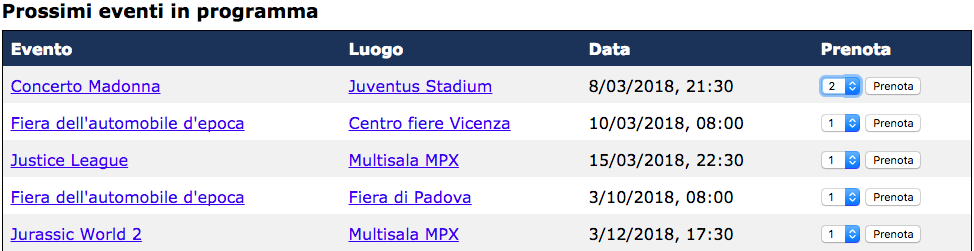
\includegraphics[width=0.65\textwidth]{Images/home_prenota.png}
  \caption{prenotazione di un biglietto direttamente in home}
  \label{fig:home_prenota}
\end{figure}

\item[\textbf{\textcolor{UniPD}{Categorie}}] (in Figura~\ref{fig:categorie}) 
visualizza tutte le categorie di eventi presenti nel sito.
Ad ogni categoria sono associate una breve descrizione ed una immagine,
in modo da chiarire la maggior parte dei dubbi che possono venire all'utente.
La pagina è generata dinamicamente dal file \emph{categorie.php}.
Cliccando sul nome di una categoria, l'utente visualizzerà una pagina 
generata dinamicamente che gli mostrerà tutti gli eventi relativi alla
categoria selezionata, se poi clicca su un evento verrà reindirizzato
ad un'altra pagina che visualizza la ''scheda dell'evento'' ovvero tutte
le informazioni ad esso relative.

\begin{figure}[h!]
  \centering
  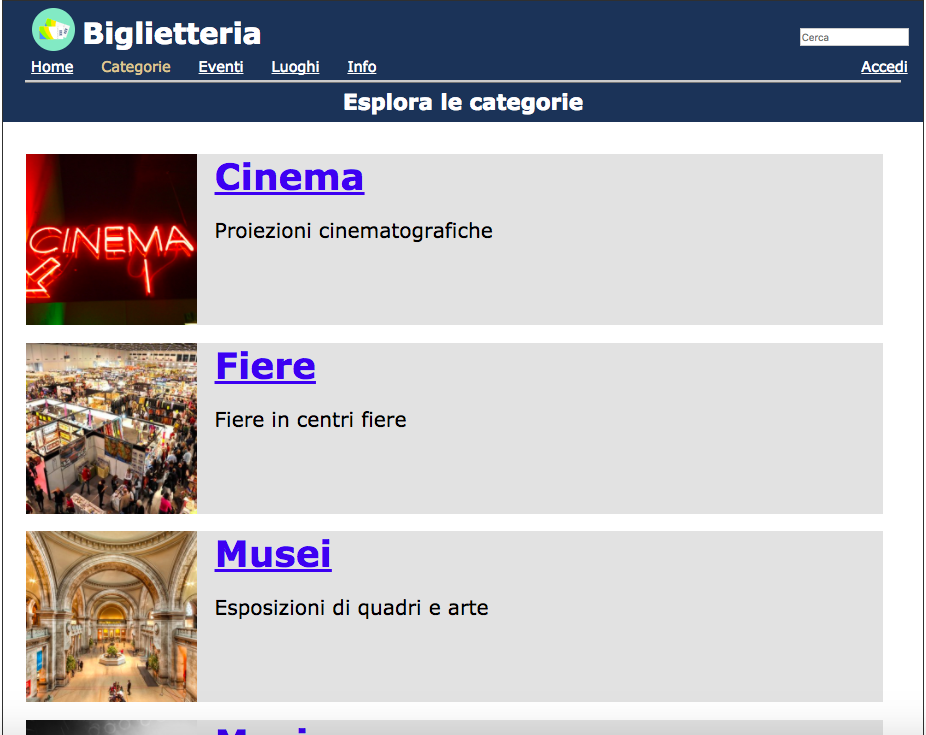
\includegraphics[width=0.65\textwidth]{Images/categorie.png}
  \caption{pagina di visualizzazione delle categorie}
  \label{fig:categorie}
\end{figure}


\item[\textbf{\textcolor{UniPD}{Eventi}}] (in Figura~\ref{fig:eventi})
visualizza tutti gli eventi di qualsiasi
categoria che sono presenti nella piattaforma. 
Oltre al nome di un evento, sono visalizzate anche la sua durata, 
la sua categoria di appartenenza ed anche la disponibilità di spettacoli.
La pagina è generata dinamicamente dal file \emph{eventi.php}.
Al caricamento della pagina gli eventi sono visualizzati secondo
uno schema di organizzazione esatto di tipo alfabetico a seconda
del loro nome. L'utente può però scegliere di ordinarli a seconda
della categoria a cui appartengono o anche a seconda della loro
durata, per farlo gli basterà cliccare le relative voci 
nell'intestazione della tabella che visualizza gli eventi
(esempio in Figura~\ref{fig:eventi_ordinati_tab}, dove
gli eventi sono ordinati per categoria).

All'utente viene offerta anche la possibilità di cercare un evento
inserendo il nome o solamente una parte di esso, nell'apposita
barra di ricerca, situata sopra la tabella di visualizzazione degli
eventi (visibile in Figura~\ref{fig:eventi_ordinati_tab}).

Se si clicca sul nome di un evento si viene reindirizzati ad una pagina
generata automaticamente che visualizza tutti gli spettacoli
di quell'evento e, se l'utente è loggato può prenotare dei biglietti
per lo spettacolo che sceglie (ad esempio in Figura~\ref{fig:evento_luogo.png}
sono visualizzati tutti gli spettacoli relativi all'evento \emph{Fiera dell'automobile d'epoca},
in questo caso ci sono due spettacoli che hanno luogo al Centro fiere Vicenza oppure alla Fiera di Padova).


\begin{figure}[h!]
  \centering
  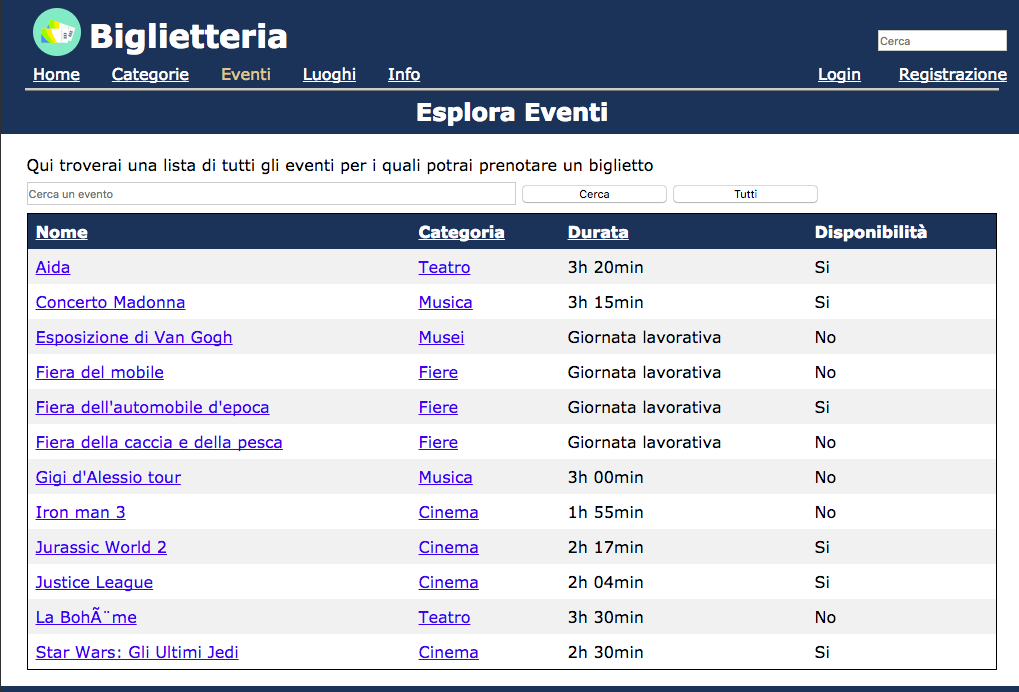
\includegraphics[width=0.65\textwidth]{Images/eventi.png}
  \caption{pagina di visualizzazione degli eventi}
  \label{fig:eventi}
\end{figure}

\begin{figure}[h!]
  \centering
  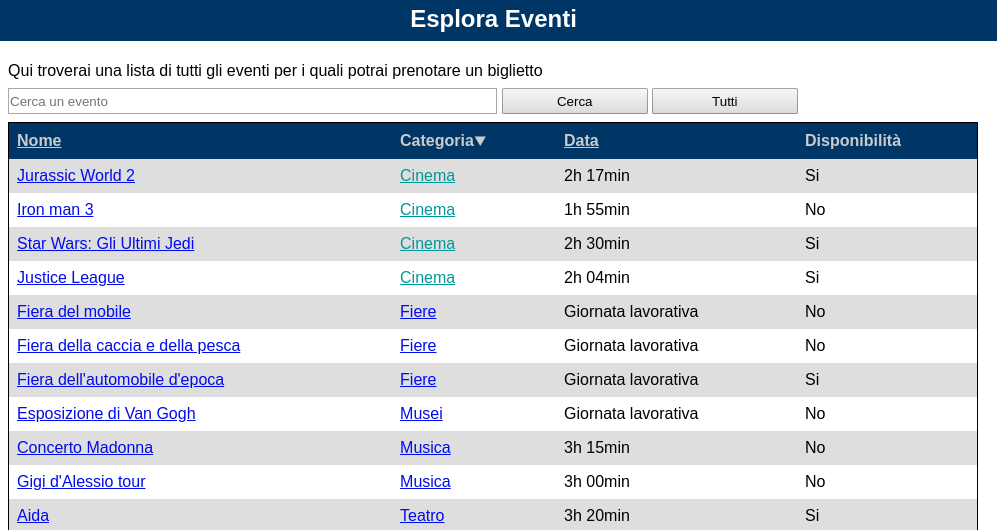
\includegraphics[width=0.65\textwidth]{Images/eventi_ordinati_tab.png}
  \caption{eventi ordinati per categoria}
  \label{fig:eventi_ordinati_tab}
\end{figure}

\begin{figure}[h!]
	\centering
	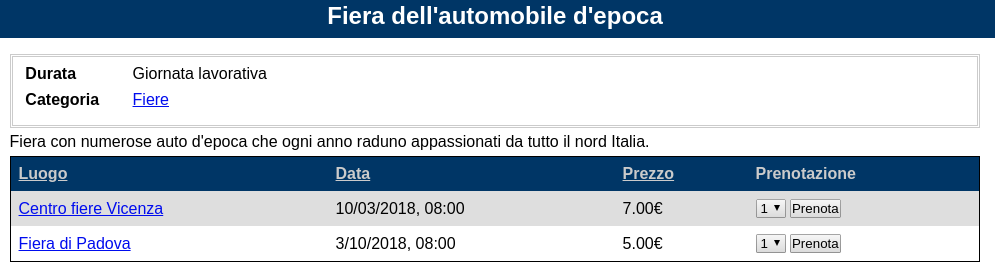
\includegraphics[width=0.75\textwidth]{Images/evento_luogo.png}
	\caption{pagina di visualizzazione degli spettacoli per l'evento Fiera dell'automobile d'epoca}
	\label{fig:evento_luogo.png}
\end{figure}

\item[\textbf{\textcolor{UniPD}{Luoghi}}] (in Figura~\ref{fig:luoghi})
visualizza l'elenco dei luoghi in cui si terranno 
gli spettacoli per i quali è possibile prenotare un biglietto.
Ad ogni luogo sono associati una descrizione ed un numero telefonico.
La pagina è generata dinamicamente dal file \emph{luoghi.php}.

Come per gli eventi, all'utente viene offerta la possibilità di cercare un luogo
inserendone il nome (o una parte di esso) nell'apposita barra di ricerca, collocata sopra
la tabella di visualizzazione dei luoghi.
\begin{figure}[h!]
  \centering
  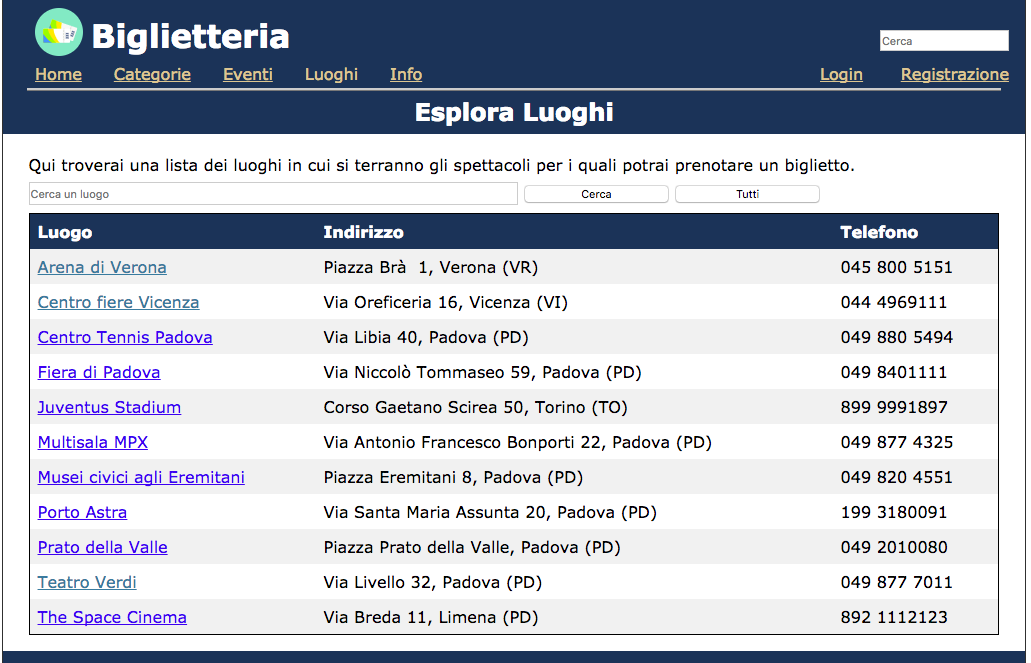
\includegraphics[width=0.65\textwidth]{Images/luoghi.png}
  \caption{pagina di visualizzazione dei luoghi}
  \label{fig:luoghi}
\end{figure}


\item[\textbf{\textcolor{UniPD}{Info}}] (in Figura~\ref{fig:info}) è un'area del sito corrispondente ad un 
''sistema di navigazione'' supplementare che può servire all'utente come guida
di usabilità e fornisce anche delle informazioni quali la missione, l'obbiettivo
e la strategia che si sono posti i creatori del sito.

\begin{figure}[h!]
	\centering
	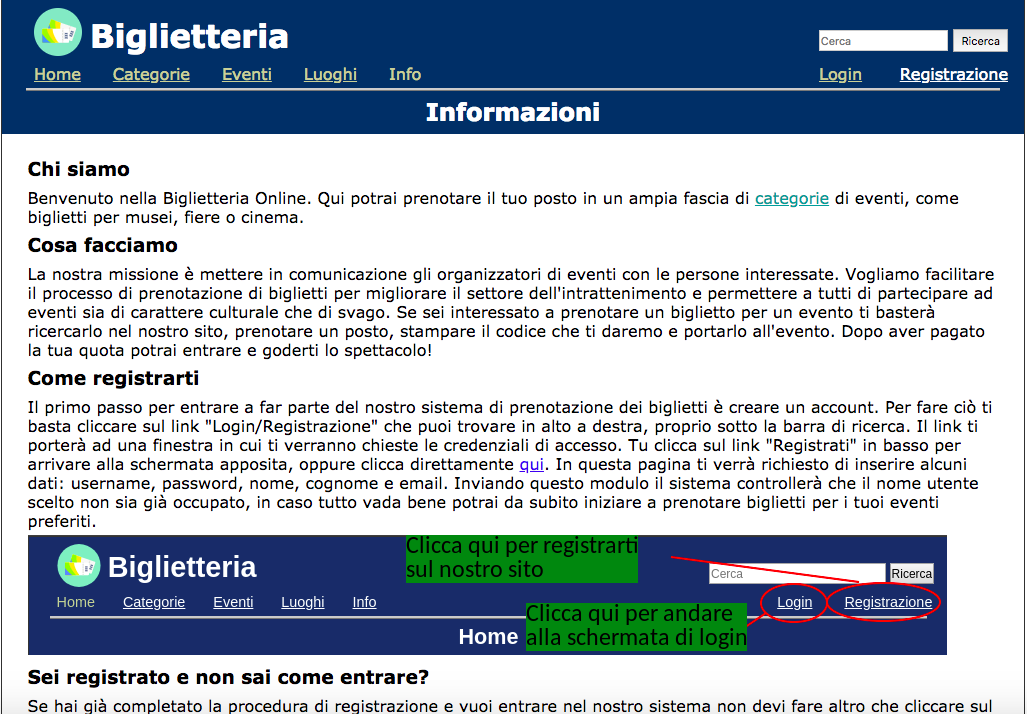
\includegraphics[width=0.65\textwidth]{Images/info.png}
	\caption{pagina di visualizzazione delle informazioni}
	\label{fig:info}
\end{figure}
\end{labeling}

\subsection{Struttura organizzativa}
É stata usata una struttura organizzativa a \textbf{database} perché ogni oggetto
informativo (un evento, una categoria, un luogo, \dots) fa parte di una collezione
di informazioni strutturata che permette di rendere ''\emph{efficaci}'' le ricerche
e le navigazioni degli utenti.

%%%%%%%%%%%%%%%%%%%%%%%%%%%%%%%%%%%%%%%%%%%%%%%%%%%%%%%%%%%%%%%%%%%%%%%%%%%%%%%%%%%%%%%%%%%%%%%%%%%

\section{Accessibilità}
Per ottenere un sito che fosse accessibile, oltre ad implementarlo cercando la massima separazione tra struttura, presentazione e contenuto abbiamo seguito alcune linee guide proposte dal W3C nell'ambito dell'iniziativa Web Content Accessibility Guidelines(WCAG), portata avanti dal WAI, una divisione del W3C che si preoccupa di migliorare l'accessibilità al web alle persone disabili. Ci siamo basati sulla versione più recente, ovvero la 2.0. Di seguito sono indicate le linee guida di WCAG2, raggruppate per "principio", con una breve spiegazione di come si è implementata la tale indicazione.

	\subsection{Perceivable}
		\subsubsection{Text alternatives}
		I contenuti non testuali dispongono di un'alternativa testuale. Così facendo, il testo può essere elaborato da dispositivi specifici che ne rielaborano il contenuto per presentarlo alle persone non vedenti. Il testo può ad esempio essere letto da uno screenreader oppure stampato in braille.
		
		\subsubsection{Time-based media}
		I contenuti temporali possono risultare poco accessibili ai disabili e quindi sarebbero da evitare, oppure da inserire evitandone però l'inizio automatico. Il nostro sito è privo di tali contenuti.
		
		\subsubsection{Easiness of distincion}
		Non abbiamo usato i colori per rappresentare le informazioni. Se si facesse uso dei colori per veicolare le informazioni queste non sarebbero accessibili da persone con disabilità visive. La maggior parte del contenuto testuale è in colore nero su sfondo bianco. Nelle tabelle lo sfondo è anche grigio chiaro.
	
	\subsection{Operable}
		\subsubsection{Keyboard}
		Si può navigare il sito, seguire i link e compilare i form attraverso la tastiera, utilizzando ad esempio il TAB.
		
		\subsubsection{Time availability}
		Nessun contenuto del sito è temporizzato. Se così non fosse tali informazioni potrebbero non essere fruibili da tutti.
		
		\subsubsection{Epilepsy}
		Il sito è privo di scritte lampeggianti per evitare di provocare attacchi epilettici.
		
		\subsubsection{Navigability}
		È presente un link al contenuto che permette agli screen reader di saltare la lettura della casella di ricerca e della barra di navigazione e di andare direttamente ai contenuti di ogni pagina. Così facendo si migliora l'esperienza di navigazione degli utenti ipovedenti.
	
	\subsection{Understandable}
		\subsubsection{Text understandability}
		Il sito è scritto in lingua italiana con codifica UTF-8. Le parole straniere, che sono solamente in lingua inglese, sono inserite come {<span lang=''en''>Foreign Word</span>}, per favorirne la traduzione dagli screenreader.
		
		\subsubsection{Predictability}
		L'aspetto del sito è uniforme. I meccanismi di navigazione sono sempre nello stesso ordine per evitare di creare confusione all'utente.
	
	\subsection{Robust}
		\subsubsection{Compatibility}
		Il sito è stato sviluppato con HTML5 e CSS3. Per l'accessibilità utilizza alcuni elementi di ARIA\cite{ARIA}. Tali tecnologie sono ben radicate e diffuse quindi il rischio vi siano incompatibilità è basso. È anche consultabile dai dispositivi più moderni.

\subsection{Esempio form}
%Inserire il form. tolto perché ogni volta che compilo mi spacco i coglioni a premere invio
\begin{lstlisting}[caption={registrazione.php},captionpos=b]
<form action="registrazione_r.php" method="POST" name="form">
	<label lang="en" for="username">Username</label>
	<input tabindex="10" id="username" type="text" name="username_r" REQUIRED />
	
	<label lang="en" for="password">Password</label>
	<input tabindex="20" id="password" type="password" name="password_r" REQUIRED />
	
	<label for="nome">Nome</label>
	<input tabindex="30" id="nome" type="text" name="nome_r"  placeholder="Inserisci il tuo nome" REQUIRED />
	
	<label for="cognome">Cognome</label>
	<input tabindex="40" id="cognome" type="text" name="cognome_r" placeholder="Inserisci il tuo cognome" REQUIRED />
	
	<label lang="en" for="email">Email</label>
	<input tabindex="50" id="email" type="email" name="email_r" placeholder="esempio@esempio.com" REQUIRED />
	
	<input type="hidden" name="tipo_r" value="U" /><hr>
	<div class="boxInline">
		<input tabindex="60" type="submit" value="Completa registrazione" />
		<input tabindex="70" id="buttonRight" type="reset" value="Azzera campi" />
	</div>
</form>
\end{lstlisting}


Si può notare in questo esempio come siano stati posti i tag di label per gli input e i tabindex. I primi permettono di facilitare la selezione del campo in cui scrivere: infatti schiacciando sul label si potrà direttamente inserire il testo nella casella apposita. Il tabindex invece permette di scorrere con il tab i vari campi. Sono stati posti con un incremento di 10 per non doverli cambiare tutti nel caso in futuro ci fosse da inserire un nuovo campo da compilare.


\subsection{Esempio tabella}
%- inserire tabellona
\begin{lstlisting}[caption={luoghi.php},captionpos=b]
<table aria-label="Tabella contenente tutti i luoghi registrati sul nostro sito" title="La seguente tabella contiene tutti i luoghi registrati sul nostro sito presso cui sono organizzati spettacoli">
	<thead>
		<tr>
			<th scope="col" >Luogo</th>
			<th scope="col" >Indirizzo</th>
			<th scope="col" >Telefono</th>
		</tr>
	</thead>
	<tbody>
	<?php
		no_result($luoghi,3);
		foreach($luoghi as $l){
			echo "<tr>";
			
			echo "<td><a title=\"Vai al luogo ".$l["nome"]."\" href="luogo_scheda.php?luogo_id=".$l["id"]."">".$l["nome"];
			echo "</a></td>";
			
			echo "<td>".$l["indirizzo"];
			echo "</td>";
			
			echo "<td>".$l["telefono"];
			echo "</td>";
		}
	?>
	</tbody>
</table> 

\end{lstlisting}


Partendo dall'alto, si può notare l'utilizzo di \texttt{aria-label}. Questo attributo fa parte di un set di attributi, denominato ARIA\cite{ARIA}, il quale è stato sviluppato per incrementare l'accessibilità del web, essendo stato costruito ad hoc per gli screen reader. È molto diffuso sia in Italia che nel mondo \cite{Diffusione ARIA}. Per venire incontro agli utenti con un browser non aggiornato è stato comunque predisposto il classico \texttt{title}. Non è stato usato \texttt{summary} in quanto non più supportato in HTML5, ed è stato scartato \texttt{caption} poichè mostrava sullo schermo una descrizione che sarebbe risultata ridondante agli utenti non disabili.
Scendendo si può notare l'utilizzo di \texttt{thead} per raggruppare gli header, che sono definiti nel tag \texttt{th}. I \texttt{th} hanno come attributo \texttt{scope="col"}, poichè definiscono il contenuto degli elementi disposti in colonna sotto di loro. Le celle contenenti i dati sono definite in \texttt{tbody} ed il loro contenuto viene stampato con degli \texttt{echo} contenuti in un ciclo \texttt{foreach} il quale prende uno ad uno i luoghi contenuti nel database (la query non è stata inclusa nello snippet) assegnati alla variabile \texttt{\$luoghi}.

\subsection{Simulazione visione di con disturbi visivi}
Abbiamo utilizzato ImageJ\cite{ImageJ} e il suo plugin Vischeck\cite{Vischeck} per simulare come appare il sito agli utenti affetti da daltonismo. Di seguito i risultati.

\subsection{Deuteranopia}
Figura~\ref{fig:ldeuteranope}
\begin{figure}[H]
	\centering
	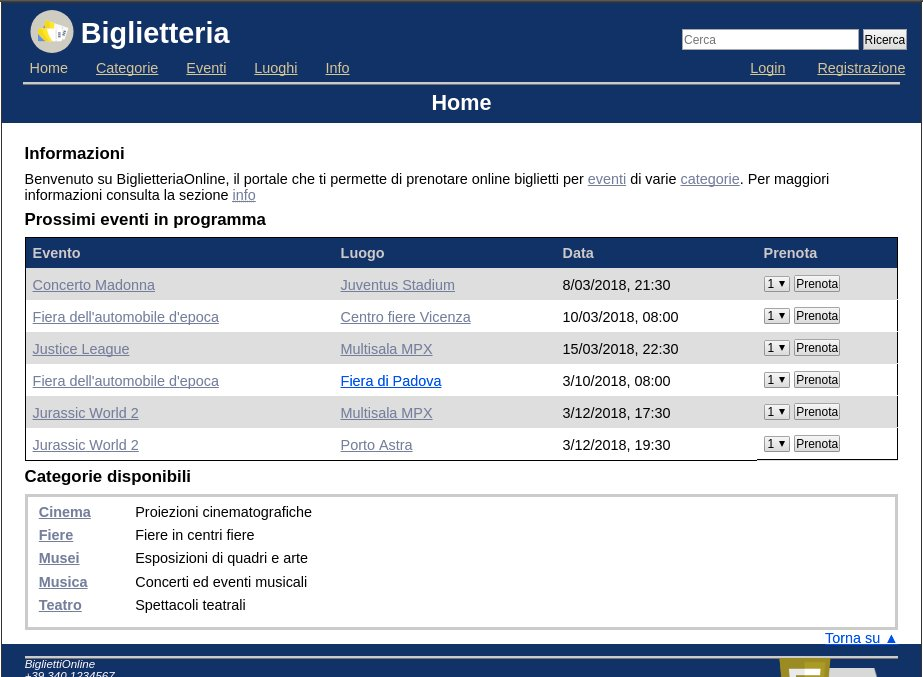
\includegraphics[width=0.65\textwidth]{Images/Deuteranope.jpg}
	\caption{Simulazione di deuteranopia}
	\label{fig:ldeuteranope}
\end{figure}


\subsection{Protanopia}
Figura~\ref{fig:protanope}
\begin{figure}[H]
	\centering
	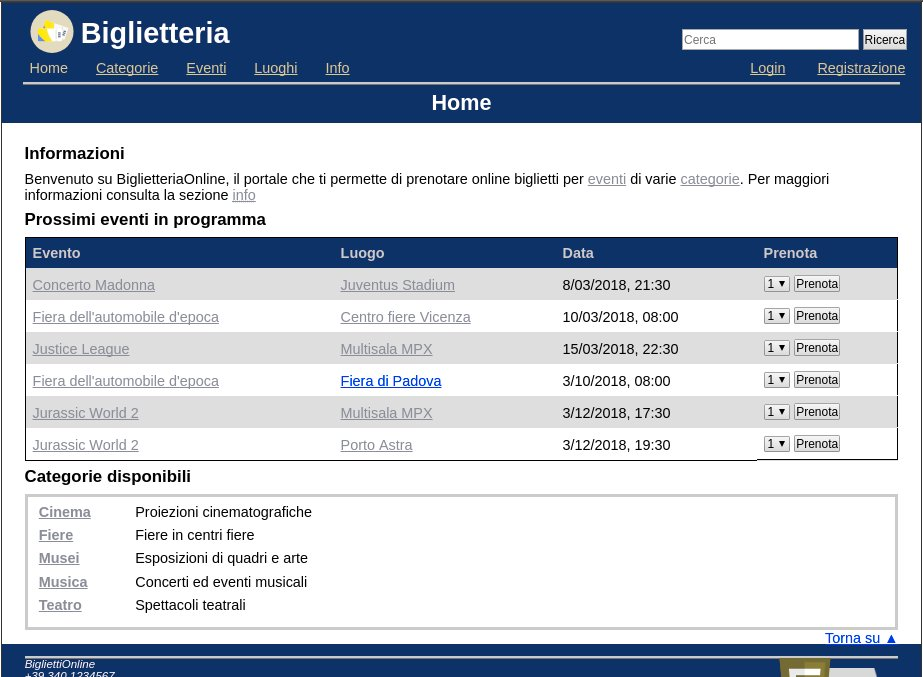
\includegraphics[width=0.65\textwidth]{Images/Protanope.jpg}
	\caption{Simulazione di protanopia}
	\label{fig:protanope}
\end{figure}


\subsection{Tritanopia}
Figura~\ref{fig:tritanope}
\begin{figure}[H]
	\centering
	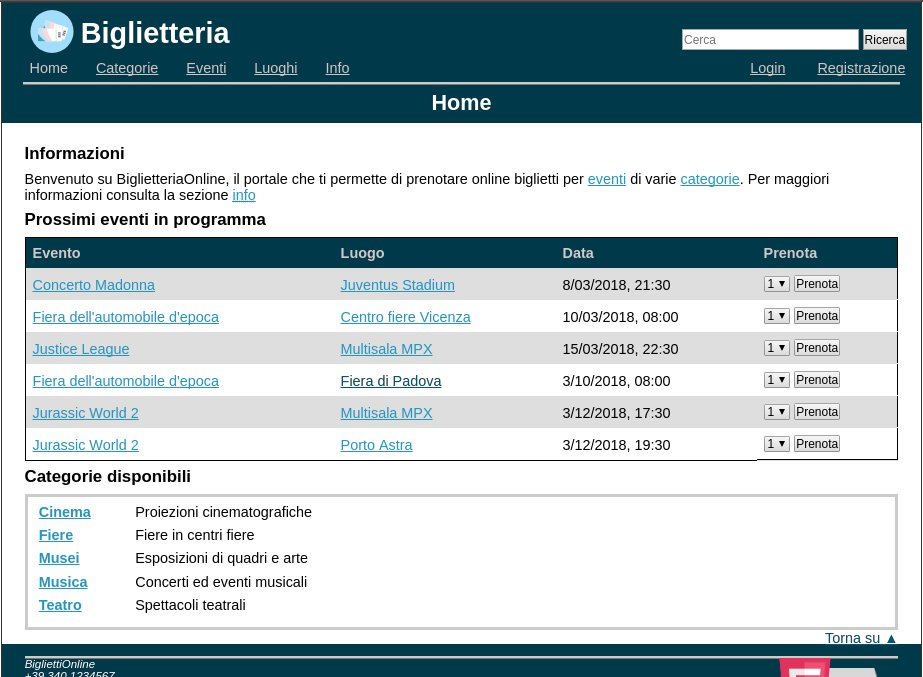
\includegraphics[width=0.65\textwidth]{Images/Tritanope.jpg}
	\caption{Simulazione di tritanopia}
	\label{fig:tritanope}
\end{figure}





\subsection{Colori web safe}
Il sito utilizza dei colori web safe, in questo modo si è sicuri che venga visualizzato correttamente
da qualsiasi utente, anche da quello con un pc così datato da essere in grado di visualizzare solamente
256 colori. I colori websafe che abbiamo usato noi, possono essere rappresentati in esadecimale
con coppie di cifre a due a due uguali (es: \#003366).
      
%%%%%%%%%%%%%%%%%%%%%%%%%%%%%%%%%%%%%%%%%%%%%%%%%%%%%%%%%%%%%%%%%%%%%%%%%%%%%%%%%%%%%%%%%%%%%%%%%%%

\section{Usabilità}
\subsection{Link}
Tutti i \textbf{link} presenti nel sito appaiono \textbf{sottolineati} in modo che l'utente sia in 
grado di accorgersi immediatamente che sono una parte del testo cliccabile.
Tutti i link cliccati assumono un colore diverso da quelli che non lo sono, in questo modo
l'utente può tenere traccia delle pagine che ha visitato e di quelle che non ha visitato.
Per quanto riguarda la barra di navigazione (navbar) i link non visitati sono visualizzati
in bianco mentre quelli visitati sono color \textcolor{Crema}{crema}. 
I link situati nella restante parte di una pagina sono di color 
\textcolor{LinkNormNoClick}{blu scuro} quando non cliccati e 
\textcolor{LinkNormClick}{azzurrino chiaro} quando lo sono.

\subsection{Navbar}
Come visibile in Figura~\ref{fig:barra_no_click}, nella barra di navigazione globale
i \textbf{link non sono circolari} perché in questo modo l'utente non si
disorienta. Se ad esempio si visita la pagina \textbf{\textcolor{UniPD}{Home}} 
(come in Figura~\ref{fig:barra_no_click}) la voce ''\textcolor{UniPD}{Home}'' della
barrà non è sottolineata, non è cliccabile ed è di color \textcolor{Crema}{crema}, questo serve per
fare capire all'utente che ha visitato almeno una volta quella pagina e che in quel
preciso momento sta visitando esattamente quella.

% \subsection{Le 5~W}
% L'homepage del sito è stata realizzata per rispondere alle classiche cinque domande
% (conosciute nel mondo anglosassone come 5~W)
% in modo da rendere fruibile l'informazione nel modo più efficace possibile.
% \begin{labeling}{alligator}
%   \item [Where? - A quale sito sono arrivato?]
%   La breve descrizione del sito contenuta nella
%   homepage (''area''  \textbf{Informazioni})permette di far capire all'utente
%   in modo veloce in che sito è arrivato. Inoltre
%   contiene un link alla pagina \textbf{\textcolor{UniPD}{Info}}.
%   \item [Who? - Chi c'è dietro questo sito?] In alto a sinistra sono presenti il logo ed il nome del sito
%     (come si puo vedere in Figura~\ref{fig:barra_no_click}), in questo modo, sin dalla
%     prima visita, l'utente comprende che si sta parlando di un sito che ha a che
%     fare con dei biglietti e vi associa anche un logo.
%     Inoltre nel footer sono presenti anche la mail, il numero di telefono e l'indirizzo
%     della biglietteria. 
%   \item [What? - Che cosa mi viene offerto?] L' ''area'' \textbf{Informazioni} collocata subito sotto alla navbar
%               \marginpar{mettere foto?}
%     spiega all'utente che il sito permette di prenotare dei biglietti per eventi
%     di varie categorie e fornisce anche un link alla pagina \textbf{\textcolor{UniPD}{Info}}
%     per spiegare meglio il tutto nel caso qualcuno non abbia capito bene o voglia approfondire.
%     Inoltre le altre ''aree'' della home \textbf{Prossimi eventi in programma} e 
%     \textbf{Categorie disponibili}, situate sotto a \textbf{Informazioni} forniscono anche
%     una panoramica sugli ultimi eventi per i quali è possibile prenotare il biglietto
%     e anche sulle categorie di eventi che sono disponibili.
%     Le varie voci della barra di navigazione fanno inoltre capire all'utente che può trovare
%     ulteriori informazioni riguardanti gli eventi e le categorie se clicca sui relativi link.
%   \item [When? - Quando?] L' ''area'' \textbf{Prossimi eventi in programma} mostra le date di
%     alcuni degli eventi in programma e quindi permette all'utente di vedere se il sito è
%     aggiornato perché, gli eventi visualizzati sono solamente quelli che non sono
%     ancora iniziati. Se non c'è alcun evento disponibile, la cosa viene segnalata.

%   \item [Why? - Perché sono qui?] La breve
%   descrizione risponde anche a questa domanda.
% \end{labeling}

\subsection{Soddisfare gli utenti}
\begin{labeling}{alligator}
  \item[Ricerca dell'oggetto conosciuto] L'utente sa cosa cercare: in questo caso dovrà semplicemente inserire ciò che desidera visualizzare nella casella di ricerca,
  collocata in alto a destra in ciascuna pagina del sito (Figura~\ref{fig:barra_ricerca}). La ricerca visualizzerà tutti i risultati corrispondenti alla richiesta effettuata dell'utente relativi agli \emph{eventi} alle \emph{categorie} ed ai \emph{luoghi}. 
  \item[Speranza di trovare cose utili durante la ricerca]
    L’utente  sta facendo una \emph{ricerca esplorativa} cercando di imparare qualche cosa.
    Ogni voce del menù può portarlo a cercare per \emph{categorie}, \emph{luoghi} o 
    \emph{eventi}.
    Se va in \emph{categorie} può selezionare quella di suo interesse e visualizzare tutti
    gli eventi che la riguardano, se va in \emph{luoghi} (Figura~\ref{fig:luoghi}) può
    cliccare su un luogo che forse gli interessa e visualizzare una pagina con le informazioni
    relative al luogo ed agli eventi che esso ospita, questi ultimi filtrabili attraverso una
    apposita barra di ricerca (Figura~\ref{fig:info_luogo}). Se infine l'utente va in
    \emph{eventi} può cliccare su un evento che potrebbe interessargli 
    (ad es. fiera dell'automobile d'epoca) e visualizzare una
    pagina con la descrizione dell'evento ed i relativi spettacoli per i quali, se è 
    loggato può prenotare direttamente dei biglietti. In tutti questi casi l'utente visualizza un ampio spettro di possibilità di scelta.

    \begin{figure}[h!]
      \centering
      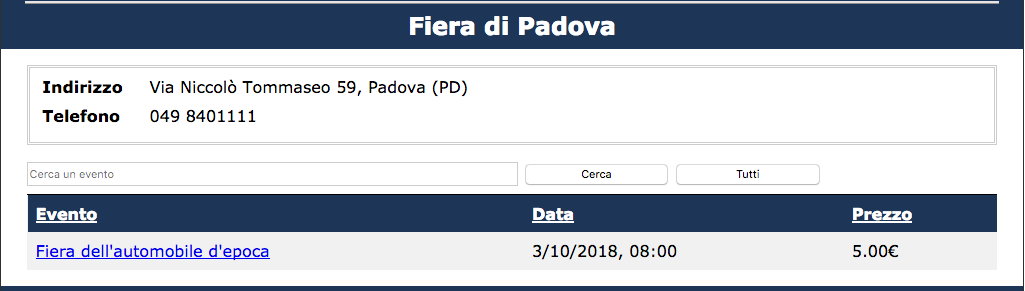
\includegraphics[width=0.75\textwidth]{Images/info_luogo.png}
      \caption{informazioni sul luogo ''fiera di padova''}
      \label{fig:info_luogo}
    \end{figure}

    \begin{figure}[h!]
      \centering
      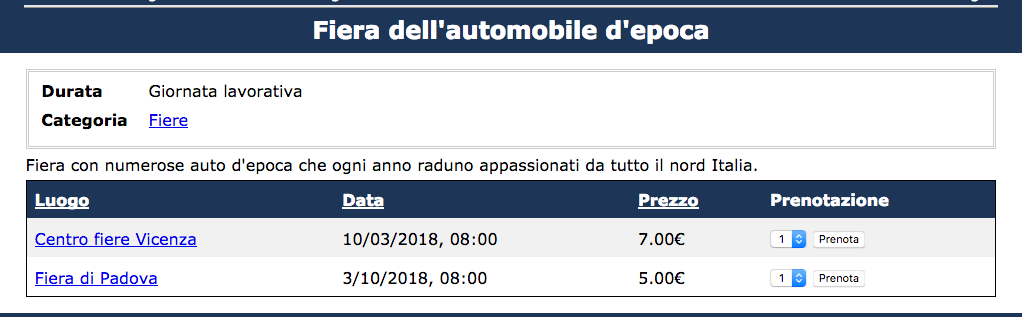
\includegraphics[width=0.75\textwidth]{Images/info_evento.png}
      \caption{informazioni sull'evento fiera delle automobili d'epoca}
      \label{fig:info_evento}
    \end{figure}

  \item[L'utente vuole tutto] L'utente vuole sapere tutto riguardo ad un 
    argomento in particolare, sta effettuando una \emph{ricerca esaustiva}
    e spera di non tralasciare niente. 
    Anche questa tipologia di navigazione può essere effettuata combinando le precedenti modalità di ricerca.

    \begin{figure}[h!]
      \centering
      
\includegraphics[width=0.35\textwidth]{Images/barra_ricerca.png}
      \caption{barra di ricerca ''globale''}
      \label{fig:barra_ricerca}
    \end{figure}

\end{labeling}

\section{Amministratore, Operatore, Amm. Luogo}
Dopo aver affettuato l'accesso (cliccando su \textbf{Login} in alto a destra, come in
Figura~\ref{fig:barra_ricerca}) l'utente ha la possibiltà di visitare il proprio profilo o di fare
il logout, gli basta cliccare su uno dei due link in alto a destra che vanno a sostituire
i precedenti \textbf{Login} e \textbf{Registrazione} e che sono rispettivamente 
un link che ha come testo quello corrispondente al nome dell'utente loggato e \textbf{Logout}
(in Figura~\ref{fig:admin_loggato} si può vedere cosa vede l'utente \emph{admin} quando loggato).
\begin{figure}[h!]
	\centering
	
\includegraphics[width=0.65\textwidth]{Images/admin_loggato.png}
	\caption{Link che vede in alto a destra l'utente admin}
	\label{fig:admin_loggato}
\end{figure}

Se l'utente clicca sul link che ha il testo corrispondente al suo nome, allora viene reindirizzato alla
pagina del suo profilo. In ogni profilo c'è un breve riepilogo dei dati dell'utente ed una tabella
che mostra lo storico  dei biglietti che sono stati prenotati per uno spettacolo e che offre la possibilità di
annullare la prenotazione per quelli che non sono ancora iniziati.

Sia gli admin che gli operatori visualizzano anche un pannello amministrazione che gli permette di compiere varie azioni di tipo amministrativo.

\subsection{Amministratore}
In Figura~\ref{fig:pannello_admin} viene mostrato il pannello dell'admin. Ogni link del pannello
permette all'admin di:
\begin{figure}[h!]
	\centering
	
\includegraphics[width=0.85\textwidth]{Images/pannello_admin.png}
	\caption{Pannello dell'amministratore}
	\label{fig:pannello_admin}
\end{figure}
\begin{labeling}{alligator}
	\item[\emph{creare una categoria}] inserendo un \emph{nome}, una \emph{descrizione} ed
	una \emph{immagine} obbligatoria.
	
	\item[\emph{creare un evento}] inserendo un \emph{nome}, una \emph{descrizione},
	la \emph{categoria} a cui appartiene e la durata. L'evento può durare tutto il giorno oppure
	può avere una durata finita ed in questo caso è necessario specificare anche quante ore e
	quanti minuti dura (un esempio di form per creare un evento è fornito in Figura~\ref{fig:creazione_evento}).
	\begin{figure}[h!]
		\centering
		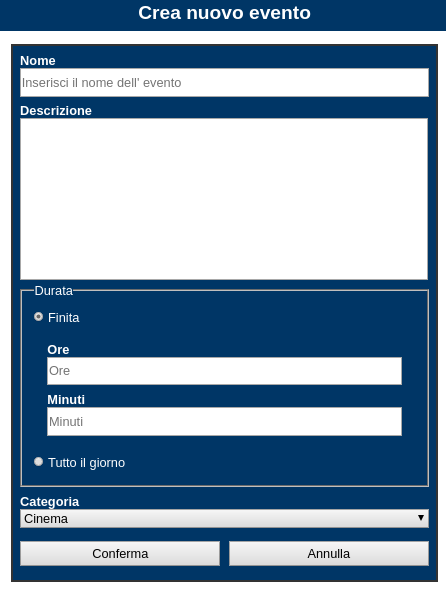
\includegraphics[width=0.65\textwidth]{Images/creazione_evento.png}
		\caption{Form per la creazione di un evento}
		\label{fig:creazione_evento}
	\end{figure}
	
	\item[\emph{creare un luogo}] inserendo \emph{nome, via, numero,
	 città, provincia}, e \emph{numero di telefono}. Inoltre è necessario
 	 creare anche un amministratore di luogo che lo amministri 
 	 (in Figura~\ref{fig:creazione_luogo} è mostrato il form di creazione di un
 	 luogo).
 	 \begin{figure}[h!]
 	 	\centering
 	 	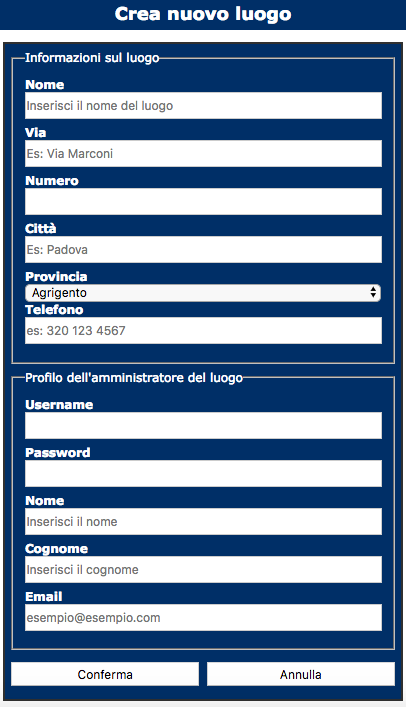
\includegraphics[width=0.65\textwidth]{Images/creazione_luogo.png}
 	 	\caption{Creazione del luogo}
 	 	\label{fig:creazione_luogo}
 	 \end{figure}
  
	\item[\emph{creare uno spettacolo}] selezionando un \emph{evento} ed un \emph{luogo}
	tra quelli disponibili, inserendo una \emph{data}, un'\emph{ora di inizio}, i \emph{posti} disponibili, 
	ed il \emph{costo} dello spettacolo (es. in Figura~\ref{fig:creazione_spettacolo}).
	\begin{figure}[h!]
		\centering
		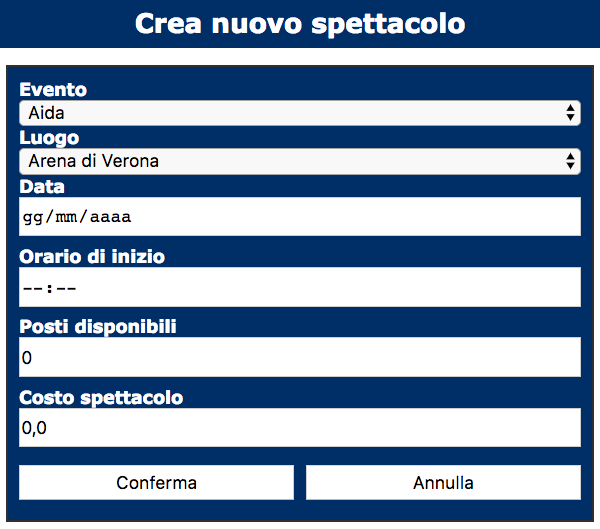
\includegraphics[width=0.65\textwidth]{Images/creazione_spettacolo.png}
		\caption{Creazione di uno spettacolo}
		\label{fig:creazione_spettacolo}
	\end{figure}
	
	\item[\emph{creare un amministratore di luogo}] permette di creare un amministratore
	per un luogo già esistente. Si noti come sia possibile avere \emph{più di un} amministratore per ogni luogo.
	
	\item[\emph{creare un operatore}] inserendo \emph{username, password, nome, 
	cognome, email}.
\end{labeling}

Oltre alle operazioni fornite dal pannello e descritte in precedenza,
un amministratore ha anche la possibilità di \textbf{modificare/eliminare una categoria},
\textbf{modificare/eliminare un evento} ed anche \textbf{modificare/eliminare un luogo}. Per farlo
deve andare nelle rispettive aree del sito (\textbf{\textcolor{UniPD}{Categorie}},
\textbf{\textcolor{UniPD}{Eventi}}, \textbf{\textcolor{UniPD}{Luoghi}},) e selezionare
la categoria/evento/luogo che intende modificare/eliminare e cliccare poi su un link
che lo reindirizzerà ad una pagina che permette di fare la modifica oppure confermare di voler eseguire l'eliminazione.

\subsection{Operatore}
Le operazioni che un operatore può svolgere sono le stesse dell'amministratore, eccezion fatta
per la possibilità di aggiungere nuovi operatori, cosa che può fare solamente l'admin.

\subsection{Amministratore luogo}
Un amministratore di luogo ha la possibilità di amministrare il luogo in cui lavora.
Dal proprio profilo, se clicca sul link \textbf{Amministra luogo} viene reindirizzato ad una pagina 
(in Figura~\ref{fig:amministrazione_porto}) che visualizza in una tabella gli spettacoli che si devono 
ancora svolgere ed in un'altra tabella più in basso tutti i biglietti prenotati dagli utenti per questi spettacoli.
Quando un utente si presenta nel luogo amministrato e acquista i biglietti prenotati
l'operatore ha il compito di segnalarlo selezionando la voce \textbf{si} nella colonna 
\textbf{utilizzato} della seconda tabella, in modo da far sapere che il codice fornito è già
stato utilizzato. Dato che il numero di biglietti prenotati può essere molto grande è anche possibile eseguire una ricerca fra di essi filtrandoli per username. Idealmente dunque un utente si presenterà alla cassa di un luogo fornendo l'username, dunque si esegue la ricerca e una volta fornito anche il codice (se esso corrisponde a quello visualizzato dal sistema) si può procedere al pagamento e l'utente può aver accesso allo spettacolo.

Se l'amministratore clicca sui link  \textit{Modifica informazioni luogo} o
\textit{Crea nuovo spettacolo} (in alto a sinistra in Figura~\ref{fig:amministrazione_porto})
può modificare le informazioni del luogo in cui lavora oppure creare un nuovo spettacolo
relativo ad un evento già esistente.

\begin{figure}[h!]
	\centering
	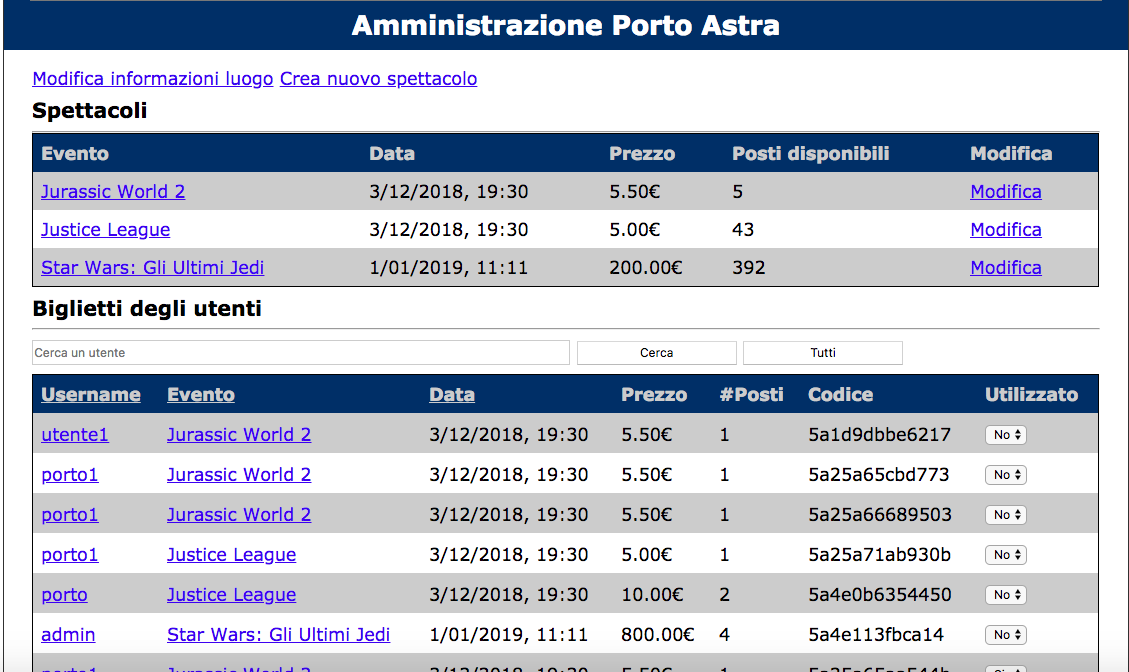
\includegraphics[width=0.65\textwidth]{Images/amministrazione_porto.png}
	\caption{Amministrazione di Porto Astra}
	\label{fig:amministrazione_porto}
\end{figure}

%%%%%%%%%%%%%%%%%%%%%%%%%%%%%%%%%%%%%%%%%%%%%%%%%%%%%%%%%%%%%%%%%%%%%%%%%%%%%%%%%%%%%%%%%%%%%%%%%%%
\section{Gerarchia dei file}
I file che compongono il sito sono contenuti nella cartella \textbf{public\textunderscore html}.
Dentro quest'ultima sono collocati tutti i file .php tranne \emph{config.php} e \emph{printTemplate.php}
che sono contenuti nella sottocartella \textbf{php}. Dentro a \textbf{public\textunderscore html} è presente
anche il file \emph{index.html}, utile perché è quello che di default ogni server web Apache visualizza se presente
nella cartella. \emph{index.html} fa un redirect a \emph{home.php}.
Di seguito sono indicate le sotto cartelle (in grassetto) ed i file che contengono:
\begin{itemize}
  \item{\textbf{css}: contiene i file css}
    \begin{itemize}
      \item{screen.css: css per gli schermi dei browser da PC}
      \item{mobile.css: css per gli schermi dei tablet e dei cellulari}
      \item{print.css: css per la stampa delle pagine}
    \end{itemize}
  \item{\textbf{img}: contiene}
    \begin{itemize}
		\item{html2.png: è l'immagine che indica che il sito è stato sviluppato con HTML5}
        \item{passv.svg: è il logo del sito}
        \item{le foto usate nell'area \textbf{\textcolor{UniPD}{Info}}}
    \end{itemize}
  \item{\textbf{immagini}: contiene le immagini corrispondenti alle categorie di eventi}
  \item{\textbf{js}: contiene il file javascript \emph{functions.js}}
\end{itemize}
%%%%%%%%%%%%%%%%%%%%%%%%%%%%%%%%%%%%%%%%%%%%%%%%%%%%%%%%%%%%%%%%%%%%%%%%%%%%%%%%%%%%%%%%%%%%%%%%%%%
\section{HTML5} \label{sec:html5}
Si è deciso di usare la tecnologia HTML5 rispetto a XHTML perché, la 
maggior parte dei membri del gruppo ha avuto già l'occasione di lavorare con XHTML
in esperienze precedenti e quindi si è preferito imparare una tecnologia nuova, mai
utilizzata da nessuno dei componenti e che sta prendendo 
piede nel mondo lavorativo. 

Una problematica nata da questa scelta è stata la grande incompatabilità delle vecchie versioni di Internet Explorer (ad esempio la 8)
con HTML5 (come si può vedere in \cite{IE supporto HTML5}). C'è da dire però che molte
proprietà non supportate non sono state usate e che prima di scegliere se usare o no
HTML5 è stata fatta una ricerca sull'utilizzo di IE. I risultati di tale ricerca dicono che solo
il $3.35\%$ della popolazione mondiale usa IE (vedere \ref{sec:compatibilita}), essendoci un
numero così ''esiguo'' di utenti che utilizzano varie versioni del browser si è deciso che l'utilizzo
di HTML5 rappresenti una scelta accettabile.

Un'altra problematica con cui si è avuto a che fare è l'incompatibilità dell'attributo \emph{time} di HTML5 con IE, Safari e le vecchie versioni di Chrome e Firefox.
Maggiori dettagli sono presenti in Sezione~\ref{sec:browser}. 
%%%%%%%%%%%%%%%%%%%%%%%%%%%%%%%%%%%%%%%%%%%%%%%%%%%%%%%%%%%%%%%%%%%%%%%%%%%%%%%%%%%%%%%%%%%%%%%%%%%
\section{PHP}
\subsection{Template di ''stampa'' delle pagine}
Il sito escludendo \textbf{index.html}, non ha alcuna pagina statica perché le altre pagine sono tutte generate dinamicamente visto che fanno uso
di funzioni di generazione della barra di navigazione, dell'header e del footer che sono
contenute nel file \emph{printTemplate.php}. In questo modo se si decide di cambiare una
''componente'' (es: la navbar), basterà modificare la funzione che la genera (\emph{printNavBar}
in questo caso) per ottenere lo stesso risultato in tutte le altre pagine del sito. La scelta di avere solamente pagine dinamiche solitamente rallenta il caricamento di esse, tuttavia non è un problema perché il sito è leggero dato che utilizza pochissime immagini e, per questo motivo non c'è alcun fattore significativo di appesantimento.

\subsection{Codice procedurale vs codice orientato agli oggetti}
Si è preferito usare uno stile procedurale di PHP rispetto ad oggetti perchè
la maggior parte delle pagine del sito effettua interrogazioni alla base di dati.
Il numero di pagine .php che compongono il sito è elevato (circa 20) e, quelle che
lavorano utilizzando il database eseguono \emph{query diverse} una dall'altra, perché
sono specializzate per eseguire specifiche operazioni.
Se fossero stati usati gli oggetti, ci sarebbe stata una sola classe che, avrebbe dovuto
contenere tutti i metodi (circa uno per ogni pagina) che effettuano le interrogazioni. Il
tutto sarebbe diventato molto difficile da gestire, inoltre, in caso di errori la
classe avrebbe dovuto visualizzare un messaggio d'errore o far morire la pagina con un
\emph{die}, cosa che non ha senso fare all'interno di una classe. Con il nostro approccio invece, questo compito viene delegato alle pagine .php
che invocano le query e che sono più adatte a gestire questo tipo di situazione perché più specializzate.


\subsection{Variabili di sessione}
Le variabili di sessione utilizzate quando un utente si logga sono:
\begin{itemize}
  \item{\textbf{user\textunderscore id}: contiene l'id dell'utente che ha effettuato il
    login (che nel database può essere trovato in una tupla della tabella \textbf{utenti}
    guardando l'attributo \textbf{id})}
  \item{\textbf{user\textunderscore username}: contiene l'username dell'utente}
  \item{\textbf{user\textunderscore tipo}: contiene il tipo dell'utente
    \emph{A},\emph{O},\emph{L},\emph{U} che sono le iniziali di 
    \emph{amministratore}, \emph{operatore}, \emph{gestore dei luoghi}, \emph{utente}}. Non è strettamente necessario avere anche questa variabile nella sessione, tuttavia essa permette di risparmiare delle queries: quando ad esempio si dovrà verificare se un utente è un amministratore, per stampare opzioni di gestione del sito, basterà leggere la variabile dalla sessione.
\end{itemize}

\subsection{config.php}
Il file \textit{config.php} contiene tutte le funzioni di utilità principali che
accedono alla base di dati, che operano sulle variabili di sessione oppure semplicemente contengono parti di codice utilizzabili da più di una pagina.

La funzione \textit{register} serve per registrare le variabili delle richieste.

\emph{Alcune} delle funzioni che hanno come compito specifico 
quello di interfacciarsi al database sono:
\begin{itemize}
  \item{query(\$sql): effettua una query usando la stringa che gli viene fornita come
    parametro utilizzando la variabile \textit{\$sql}.}
  \item{select(\$sql): Come la precedente, solamente che il risultato viene ritornato
    in una tabella}
  \item{get\textunderscore nome\textunderscore evento(\$id): ritorna il nome 
    dell'evento con un certo id}
  \item{evento\textunderscore has\textunderscore spettacoli(\$eventoid):
    ritorna true $\iff$ esiste almeno uno spettacolo associato all'evento che si cerca, altrimenti false}
\end{itemize}

La funzione \textit{redirect(\$url)} serve alle varie pagine che la utilizzano per fare
un redirect ad una pagina .php il cui nome è specificato nella variabile \textit{\$url}.

Ci sono poi delle funzioni booleane che servono per capire che tipo di utente è loggato:
\begin{itemize}
  \item{is\textunderscore admin}
  \item{is\textunderscore gestore\textunderscore luogo}
  \item{is\textunderscore operatore}
\end{itemize}

Tra le altre funzioni di utilità contenute nel file, ci sono quelle che fanno dei controlli
sui formati delle date, della valuta, \dots Risultano utili in quanto il sistema si deve interfacciare con un database e serve un metodo rapido per la conversione della rappresentazione di dati in formati diversi.

Per una lista esaustiva delle funzioni consultare il file \emph{config.php}, nel quale è presente sopra ciascuna funzione una breve descrizione. 

\subsection{printTemplate.php}
Il file \textit{printTemplate.php} contiene delle funzioni di utilità che generano
la navbar, l'header ed il footer. É incluso da ogni singola pagina che genera del
contenuto visualizzato da un qualsiasi utente. Le funzioni sono:
\begin{itemize}
  \item{printHead(\$title): stampa il contenuto del tag <head> html}
  \item{printHeader: stampa l'header della pagina (logo, scritta \textbf{Biglietteria} e la casella di ricerca globale)}
  \item{printNavBar: stampa la barra di navigazione globale}
  \item{printFooter: stampa il footer della pagina}
\end{itemize}

\subsection{Altri file PHP}
I seguenti file .php sono quelli che generano le pagine principali del sito:
\begin{itemize}
  \item{home.php}
  \item{categorie.php}
  \item{eventi.php}
  \item{luoghi.php}
  \item{info.php}
\end{itemize}
%%%%%%%%%%%%%%%%%%%%%%%%%%%%%%%%%%%%%%%%%%%%%%%%%%%%%%%%%%%%%%%%%%%%%%%%%%%%%%%%%%%%%%%%%%%%%%%%%%%
\section{Javascript}
\subsection{Utilizzo obbligatorio di Javascript}
L'admin, gli operatori e gli amministratori di luogo devono avere
Javascript abilitato nei propri browser, altrimenti il sito non funziona nel modo corretto.

In particolare la stampa della casella di inserimento della durata di un evento viene fatta utilizzando Javascript per non confondere l'utente: se si seleziona durata finita allora è possibile inserire ore e minuti, invece se si sceglie 'Tutto il giorno' non deve essere possibile inserire nient'altro.

Anche gli amministratori di luogo \emph{devono} avere Javascript abilitato perché quando un utente
si presenta nel luogo e acquista i biglietti, devono selezionare la voce \textbf{si} nella colonna 
\textbf{utilizzato} della tabella \textbf{Biglietti degli utenti}, (in Figura~\ref{fig:amministrazione_porto})
questa azione non viene \emph{eseguita} se non c'è Javascript, dato che per evitare di dover ricaricare la pagina troppe volte si è scelto eseguire una richiesta \textbf{AJAX}.

Ci rendiamo conto che questa sia una limitazione all'accessibilità, tuttavia ci è sembrata una scelta sensata, in quanto le uniche categorie a cui viene \emph{richiesto} di avere Javascript abilitato sono quelle su cui abbiamo il pieno controllo: amministratori ed operatori sono interni al sistema e dunque abbiamo il pieno controllo di essi  (dato che gli operatori sono impiegati di ''BiglietteriaOnline'' e che un luogo prima di diventare partner del sito deve farne richiesta). Poiché si ha il controllo su questi utenti, si può richiedere che Javascript sia abilitato sul browser che loro utilizzano. Questa richiesta comunque non dovrebbe rappresentare un problema, dato che presumibilmente se si desidera diventare nostri partner e \emph{informatizzare} il sistema di prenotazione dei biglietti si disporrà di apparecchiature relativamente nuove. Il fatto che sia richiesto Javascript viene comunque chiarito nella pagina \emph{info.php} dove si spiega come richiedere di diventare amministratori di luoghi partner della piattaforma.

\subsection{Javascript per l'utente ''normale''}
Se l'utente normale non ha attivato Javascript nel proprio browser riescesce comunque a navigare
senza problemi sfruttando al massimo le funzionalità che il sito gli offre.

%%%%%%%%%%%%%%%%%%%%%%%%%%%%%%%%%%%%%%%%%%%%%%%%%%%%%%%%%%%%%%%%%%%%%%%%%%%%%%%%%%%%%%%%%%%%%%%%%%%
\section{Compatibilità browser} \label{sec:compatibilita}
L'eterogeneità dei sistemi operativi usati dai membri del gruppo ha permesso di
testare il sito web su sistemi GNU/Linux, MAC OS e Windows.
Per questo motivo il sito web è stato testato facendo uso dei seguenti browser web:
Mozilla Firefox, Google Chrome, Microsoft Edge e Safari.

Per quanto riguarda i browser mobile il sito è stato testato su Google Chrome
da un ASUS ZenFone 2 Laser, non incorrendo in problemi di usabilità.

\subsection{Attributo time} \label{sec:browser}
L'admin, l'operatore e gli amministratori di luogo possono creare e modificare
uno spettacolo relativo ad un evento (es. in Figura~\ref{fig:creazione_spettacolo}).
Per permettere di inserire l'ora di inizio dello spettacolo è stato usato un tag <input> con attributo type uguale a \textbf{''time''}.
É quindi essenziale che l'admin, l'operatore e gli amministratori utilizzino come browser
Chrome (dalla versione 20 in poi), Firefox (dalla versione 57) oppure Edge (dalla versione 12).
Safari ed IE purtroppo non sono supportati, per questo motivo (come per l'abilitazione
di Javascript nel browser) è necessario che chi esegue tali operazioni utilizzi un browser che supporta tale attributo.
Ci rendiamo conto che anche questa sia una limitazione all'accessibilità, tuttavia le uniche categorie a cui viene \emph{richiesto} 
di non usare IE o safari sono quelle su cui abbiamo un controllo diretto: amministratore, operatore, amministratore di luogo.
Un utente comune può navigare con Safari o IE11 sul sito senza alcuna problematica.

Ulteriori informazioni sull'attributo time si possono trovare in \cite{time}.


\subsection{Compatibilità con IE} \marginpar{\dbend}
Per ciò che è stato detto in Sezione~\ref{sec:html5}, i vecchi browser della ''famiglia'' Internet Explorer non sono supportati completamente ma,
secondo il sito \url{http://gs.statcounter.com/} l'utilizzo globale di IE a Dicembre 2017 è inferiore al $3.50\%$ (Figura~\ref{fig:stat_brws}).

\begin{figure}[h!]
	\centering
	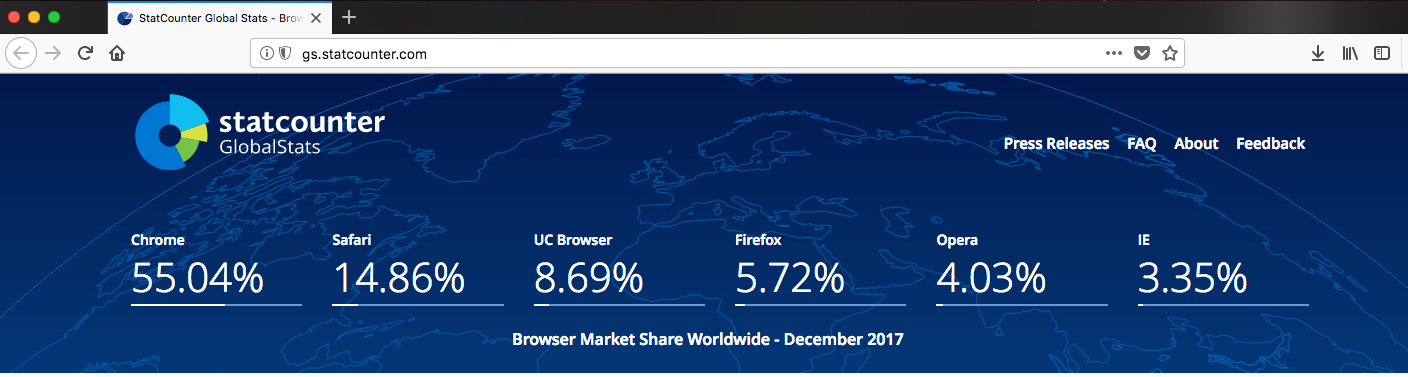
\includegraphics[width=0.80\textwidth]{Images/stat_brws.png}
	\caption{Statistiche utilizzo browser dicembre 2017}
	\label{fig:stat_brws}
\end{figure}

\subsubsection{Internet Explorer 8}
Come visibile (in Figura~\ref{fig:home_IE}) in IE 8 Il logo, la navbar i colori dei link e delle varie componenti
della pagina non sono visualizzati correttamente. Anche il footer (in Figura~\ref{fig:footer_IE}) non viene 
visualizzato nel giusto modo.
Le varie funzioni di ricerca (''globale'', degli eventi e dei luoghi)  funzionano senza presentare alcun problema.
É garantita la funzione di prenotazione dei biglietti. Le categorie sono visualizzate in modo corretto.

\begin{figure}[h!]
	\centering
	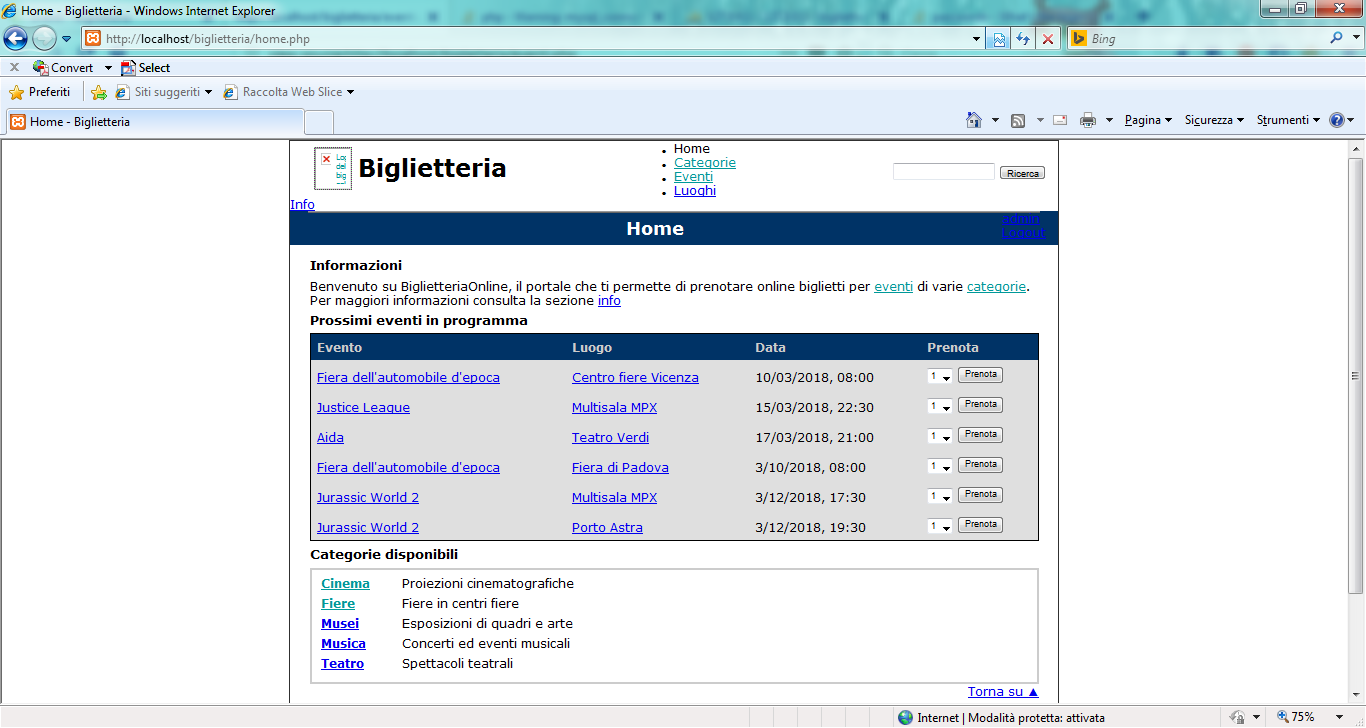
\includegraphics[width=0.65\textwidth]{Images/home_IE.png}
	\caption{Home in IE 8}
	\label{fig:home_IE}
\end{figure}

\begin{figure}[h!]
	\centering
	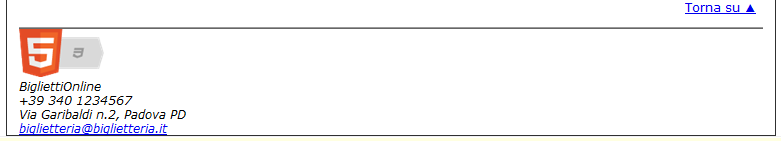
\includegraphics[width=0.65\textwidth]{Images/footer_IE.png}
	\caption{Footer in IE 8}
	\label{fig:footer_IE}
\end{figure}

\subsubsection{Internet Explorer 11}
Il sito visualizza correttamente su Internet Explorer 11 \footnote{testato dai PC in laboratorio} (come si può vedere dalla Figura~\ref{fig:IE_11}).
L'attributo time non è supportato e quindi l'amministratore deve accertarsi che gli operatori e gli amministratori di luogo 
non utilizzino IE11 e nemmeno le sue versioni precedenti come browser.
\begin{figure}[h!]
	\centering
	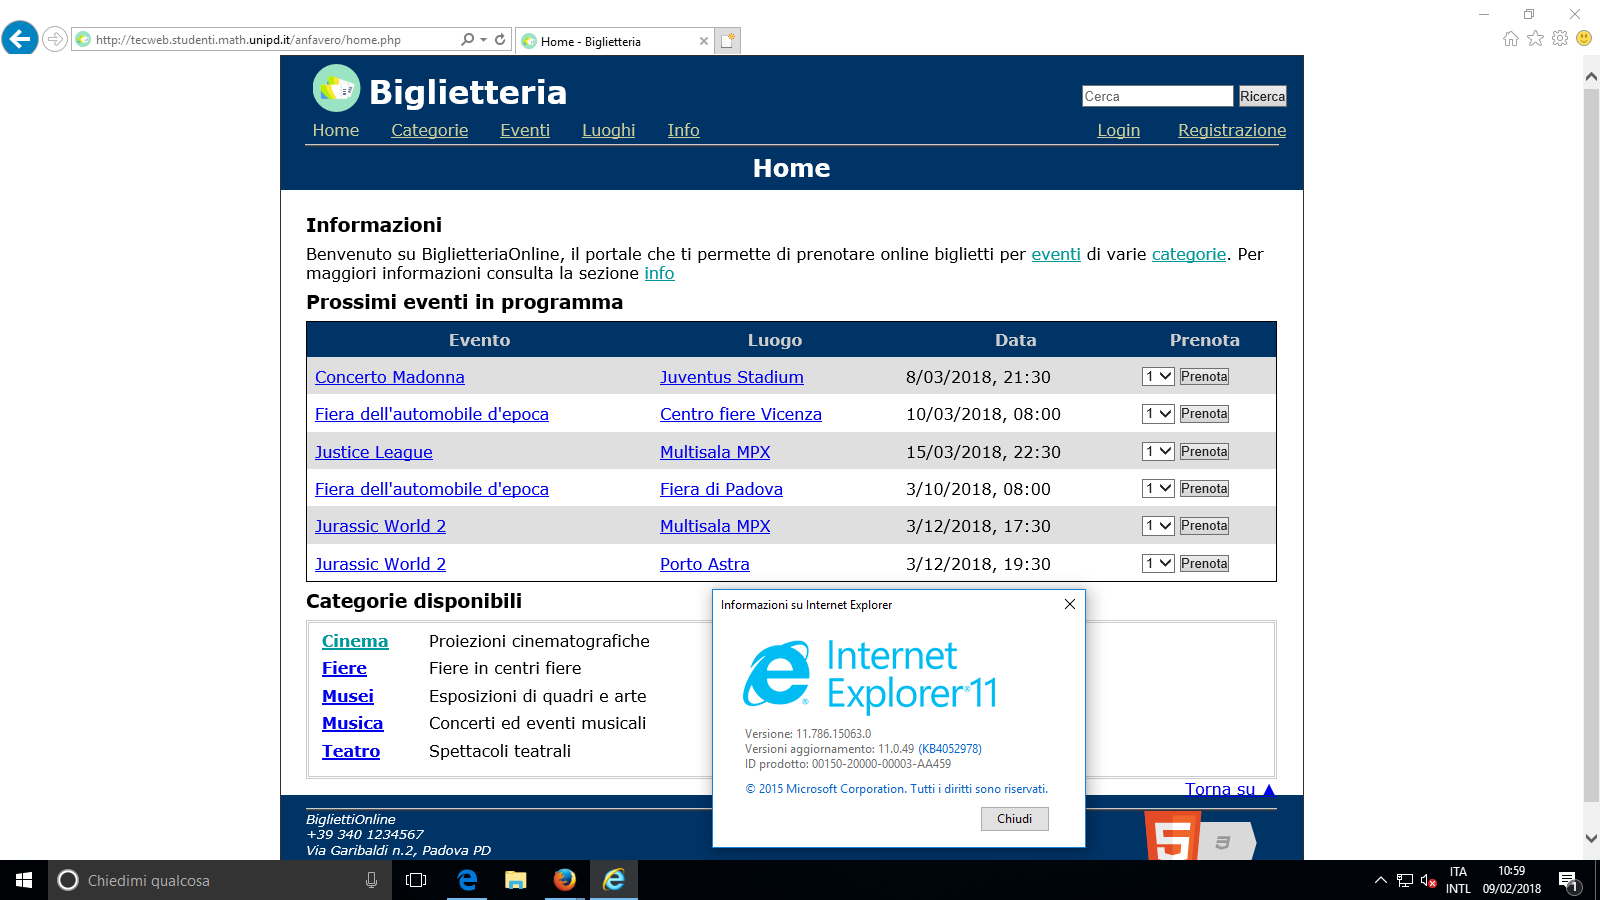
\includegraphics[width=0.65\textwidth]{Images/IE_11.png}
	\caption{Visualizzazione della home in IE 11}
	\label{fig:IE_11}
\end{figure}

\subsection{Microsoft Edge}
Il sito viene visualizzato e funziona correttamente ed è stato testato nei PC del laboratorio 
(Figura~\ref{fig:edge}) e nei PC dei componenti del gruppo che hanno Windows 10 installato.
\begin{figure}[h!]
	\centering
	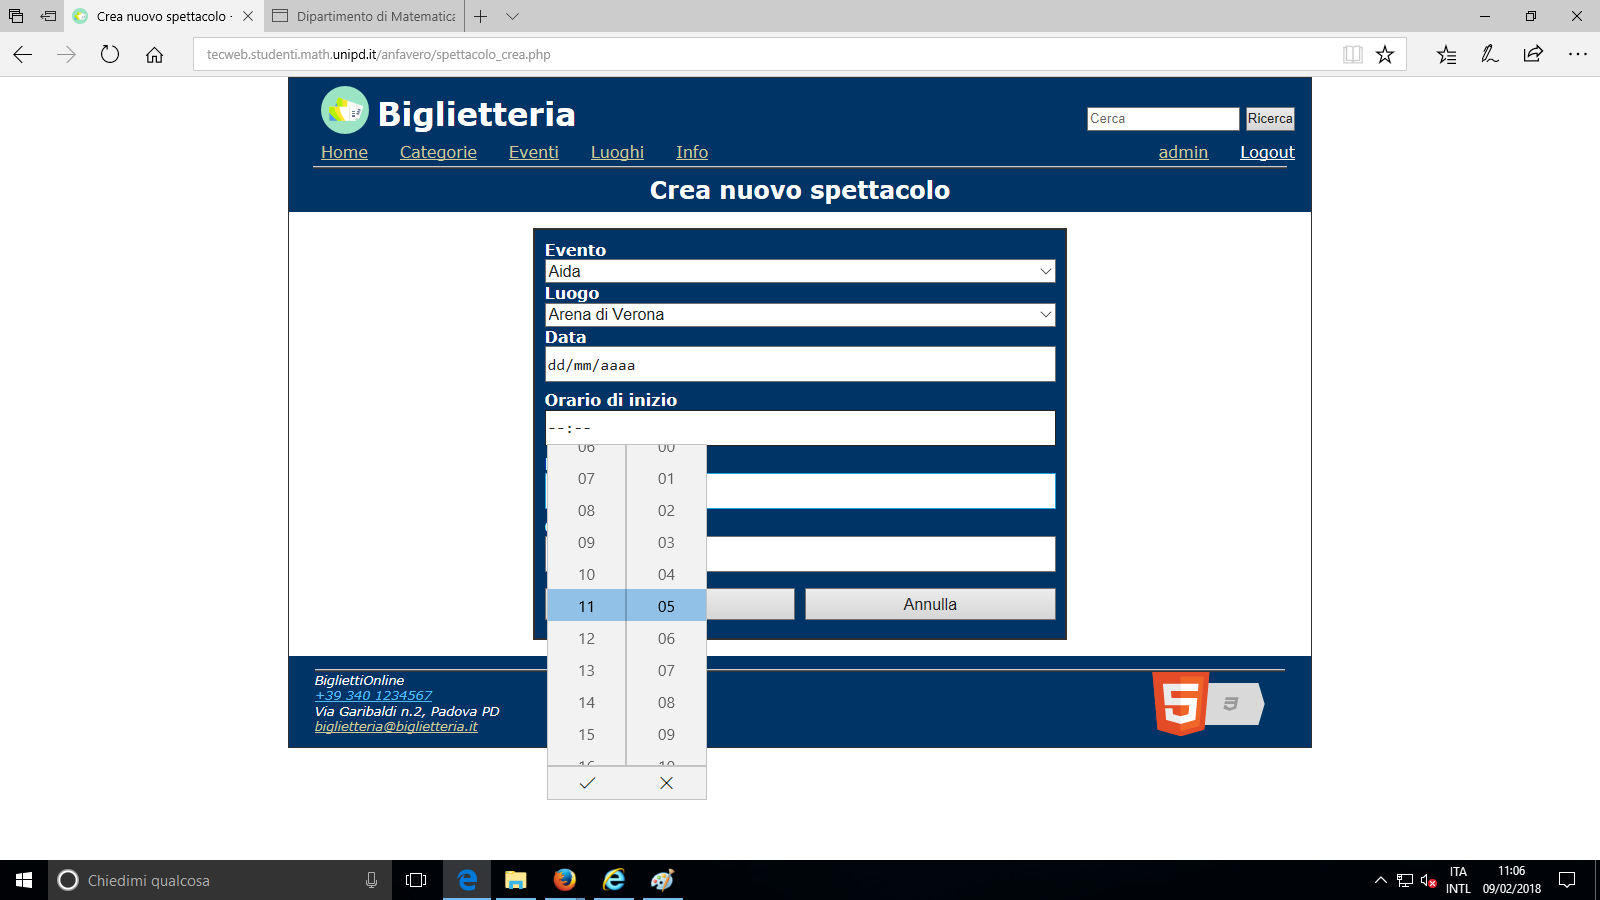
\includegraphics[width=0.65\textwidth]{Images/edge.png}
	\caption{Visualizzazione della creazione di uno spettacolo su Edge}
	\label{fig:edge}
\end{figure}

\subsection{Compatibilità con Safari} \marginpar{\dbend}
L'attributo time non è supportato e quindi l'amministratore deve accertarsi che gli operatori e gli amministratori di luogo 
non utilizzino safari. L'utente normale può navigare tranqullamente. I test sono stati effettuati sulla versione 11.0.1
del browser.

I bottoni dei form sono diversi da quelli ''standard'' che sono visualizzati correttamente in Firefox, Edge, Chrome e IE11 
per Windows.

\subsection{Compatibilità con Firefox}
\begin{labeling}{alligator}
	\item[MACOS] \item[]
		\begin{itemize}
			\item{Tutti i bottoni (anche quello della ricerca globale) sono diversi da quelli "standard" visualizzati su windows}
		\end{itemize}
	
	\item[Ubuntu] \item[]
	\begin{itemize}
		\item{Il bottone della ricerca globale è diverso da quello "standard" visualizzato in IE11, Edge e Chrome}
	\end{itemize}
\end{labeling}

\subsection{Compatibilità con Chrome}
Il sito viene visualizzato e funziona correttamente sulle versioni di Google Chrome installate nei laboratori e nei PC di tutti e 4 i
membri del gruppo. Perché l'attributo time sia supportato è necessario utilizzare una versione successiva alla 20, in questo
momento l'ultima resa disponibile è la 64.

Nelle versioni MAC i bottoni (escluso quello della ricerca globale) sono diversi da quelli "standard" visualizzati correttamente dalle versioni
di Chrome per gli altri sistemi operativi.

\subsection{Dispositivi Mobile}
I css sono stati strutturati in maniera tale da rendere il sito il più responsive possibile. Per questo motivo esistono un
foglio di stile \emph{screen.css} che è la versione per i dispositivi desktop, ed un foglio 
di stile \emph{mobile.css} che, setta una larghezza massima di 768px e che serve per 
rendere accessibile il sito ai dispositivi mobile e tablet.

In Figura~\ref{fig:firefox_zen} è mostrata la visualizzazione del sito dal browser Chrome installato su un dispositivo
ASUS ZenFone 2 laser.
\begin{figure}[h!]
	\centering
	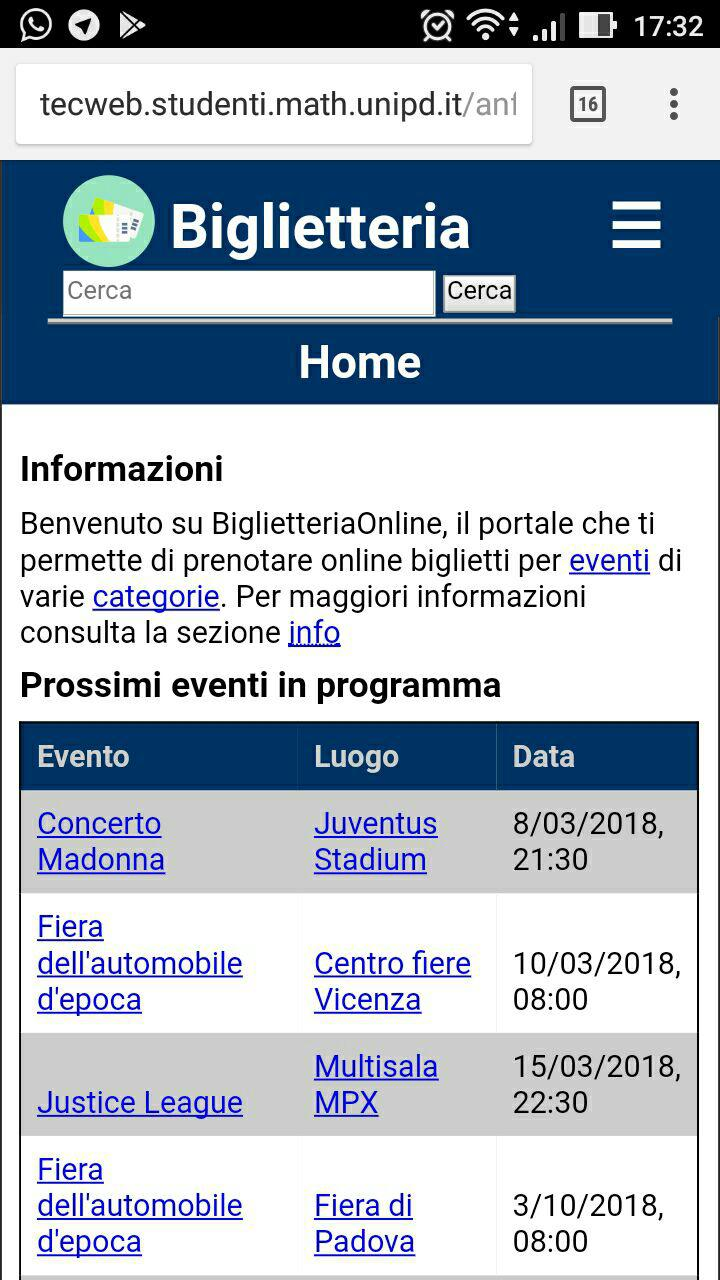
\includegraphics[width=0.45\textwidth]{Images/firefox_zen.jpg}
	\caption{Visualizzazione su Firefox installato su uno ZenFone 2 Laser}
	\label{fig:firefox_zen}
\end{figure}
%%%%%%%%%%%%%%%%%%%%%%%%%%%%%%%%%%%%%%%%%%%%%%%%%%%%%%%%%%%%%%%%%%%%%%%%%%%%%%%%%%%%%%%%%%%%%%%%%%%
\section{Validazione}
Il progetto è stato testato da tutti i componenti del gruppo utilizzando i browser installati sulle proprie macchine ed anche
quelli presenti nei PC del laboratorio informatico di Torre Archimede.
Sono stati fatti dei test usando anche il browser testuale \textbf{Lynx} e la carta stampata,
quest'ultima è stata molto utile perché ci ha permesso di controllare che i link fossero visibili
in maniera immediata all'utente.\\
Sono stati utilizzati i validatori della W3C per verificare che l'HTML
(\url{https://validator.w3.org}) ed i CSS (\url{https://jigsaw.w3.org/css-validator/})
utilizzati fossero conformi agli standard.

\section{Suddivisione del lavoro tra i componenti del gruppo}
\begin{labeling}{alligator}
	\item[Andrea Favero] \item[] %serve perché altrimenti il primo elemento della lista inizia su questa linea
		\begin{itemize}
			\item{\textbf{CSS}: creazione dei CSS per le tabelle.}
			\item{\textbf{PHP}: lavoro su alcuni file, ad esempio quelli riguardanti il
			caricamento e la modifica di una categoria.}
			\item{\textbf{Configurazione sturmenti:} predisposizione strumenti per lavorare in locale e
			delle configurazioni per la consegna del progetto.}
			\item{\textbf{Test:} browser su MAC OS, Chrome su dispositivi mobili.}
		\end{itemize}
	\item[Cristian Maschio] \item[]
		\begin{itemize}
			\item{\textbf{CSS}: creazione dei file CSS per desktop, mobile, e stampa.}
			\item{\textbf{Database}: popolazione del database.}
			\item{\textbf{PHP}: lavoro su alcuni file.}
			\item{\textbf{Test:} Microsoft Edge tramite macchine laboratorio e proprio
				PC portatile, Firefox su Windows 10.}
		\end{itemize}
	\item[Francesco Parolini] \item[]
		\begin{itemize}
			\item{\textbf{PHP}: scrittura della maggioranza dei file php.}
			\item{\textbf{Javascript}: scrittura delle funzioni Javascript.}
			\item{\textbf{Test:}  Chrome su Windows.}
		\end{itemize}
	\item[Paolo Eccher] \item[]
		\begin{itemize}	
			\item{\textbf{PHP}: scrittura di alcuni file PHP.}
			\item{\textbf{Accessibilità}: rese accessibili le pagine del sito lavorando su praticamente tutti i file php.}
			\item{\textbf{Test:}  Chrome su Linux.}
		\end{itemize}
\end{labeling}
Inoltre, tutti i componenti del gruppo hanno contribuito a redigere la relazione.

\begin{thebibliography}{9}
	
	\bibitem{time}
	<input type="time"> Mozilla Developers Network
	\textit{\url{https://developer.mozilla.org/en-US/docs/Web/HTML/Element/input/time}}
	
	\bibitem{ImageJ}
	Image Processing and Analysis in Java
	\textit{\url{https://imagej.nih.gov/ij/}}
	
	\bibitem{Vischeck}
	Vischeck official website
	\textit{\url{http://www.vischeck.com/}}
	
	\bibitem{IE supporto HTML5}
	HTML5test - How well does your browser support HTML5?
	\textit{\url{https://html5test.com/compare/browser/ie-10.html}}
	
	\bibitem{ARIA}
	ARIA - Accessible Rich Internet Applications
	\textit{\url{https://developer.mozilla.org/en-US/docs/Web/Accessibility/ARIA}}

	\bibitem{Diffusione ARIA}
	Diffusione ARIA
	\textit{\url{https://caniuse.com/\#search=aria}}
\end{thebibliography}

\end{document}
%%%%%%%%%%%%%%%%%%%%%%%%%%%%%%%%%%%%%%%%%%%%%%%%%%%%%%%%%%%%%%%%%%%%%%%%%%%%%%%%%%%%%%%%%%%%%%%%%%%%%%%%

